\documentclass[a4paper]{article}

% CJK support: prefer ctex, fallback to XeTeX native line breaking
\IfFileExists{ctex.sty}{
  \usepackage[fontset=fandol]{ctex}
}{
  % Fallback for minimal TeX installs (e.g. MacTeX Basic, TeX Live scheme-basic)
  % without ctex/xeCJK. Uses XeTeX's built-in CJK line breaking.
  \usepackage{fontspec}
  \XeTeXlinebreaklocale "zh"
  \XeTeXlinebreakskip = 0pt plus 1pt
  \IfFontExistsTF{Songti SC}{\setmainfont{Songti SC}}{%
    \IfFontExistsTF{Noto Serif CJK SC}{\setmainfont{Noto Serif CJK SC}}{}%
  }
  \IfFontExistsTF{Heiti SC}{\setsansfont{Heiti SC}}{%
    \IfFontExistsTF{Noto Sans CJK SC}{\setsansfont{Noto Sans CJK SC}}{}%
  }
}

% Basic packages
\usepackage{amsmath, amssymb}
\usepackage{graphicx}
\usepackage[margin=2.5cm]{geometry}
\emergencystretch=3em
\usepackage[most]{tcolorbox}
\usepackage{etoolbox}
\usepackage{listings}
\usepackage{hyperref}
\usepackage{booktabs}
\usepackage{array}
\usepackage{subcaption}
\usepackage{float}
\usepackage{tikz}
\IfFileExists{pgfplots.sty}{
    \usepackage{pgfplots}
    \pgfplotsset{compat=1.18}
}{}

% ===== Highlight boxes =====
\newtcolorbox{knowledgebox}[1]{
    enhanced, colback=blue!5!white, colframe=blue!75!black, colbacktitle=blue!75!black,
    coltitle=white, fonttitle=\bfseries, title={#1}, attach boxed title to top left={yshift=-2mm, xshift=2mm},
    boxrule=1pt, sharp corners
}

\newtcolorbox{importantbox}[1]{
    enhanced, colback=yellow!10!white, colframe=yellow!80!black, colbacktitle=yellow!80!black,
    coltitle=black, fonttitle=\bfseries, title={#1}, sharp corners
}

\newtcolorbox{warningbox}[1]{
    enhanced, colback=red!5!white, colframe=red!75!black, colbacktitle=red!75!black,
    coltitle=white, fonttitle=\bfseries, title={#1}, sharp corners
}

\newtcolorbox{practicebox}[1]{
    enhanced, colback=black!3!white, colframe=black!75, colbacktitle=black!75,
    coltitle=white, fonttitle=\bfseries, title={#1}, sharp corners
}

% ===== Code listings =====
\lstset{
    basicstyle=\ttfamily\small,
    keywordstyle=\color{blue},
    stringstyle=\color{red!60!black},
    commentstyle=\color{green!60!black},
    breaklines=true,
    frame=single,
    numbers=left,
    numberstyle=\tiny\color{gray},
    captionpos=b,
    extendedchars=false
}

% ===== Figure provenance and unit macros =====
% \vtag goes inside \caption{...}; \srcnote{MM:SS--MM:SS} follows the figure environment.
\newcommand{\vtag}{\protect\footnotemark}
\newcommand{\srcnote}[1]{\footnotetext{视频画面时间区间：#1。若为裁剪图，时间区间仍对应原视频画面。}}
% Units work in text and math mode; never hand-write $^\circ$ or \AA inside \mathrm.
\newcommand{\degC}{\ensuremath{^{\circ}\mathrm{C}}}
\newcommand{\um}{\ensuremath{\mu\mathrm{m}}}
\newcommand{\nm}{\ensuremath{\mathrm{nm}}}
\newcommand{\angstrom}{\ensuremath{\text{\AA}}}

% ===== Front-page metadata =====
% Fill these in when generating notes.
\newcommand{\notetitle}{计算几何}
\newcommand{\notesubtitle}{GAMES001 图形学中的数学 · 第 3 集：点线面、距离与相交、多边形、凸包、最小圆覆盖与反演}
\newcommand{\noteauthors}{根据 GAMES-Webinar 直播录像整理（倪星宇 主讲）}
\newcommand{\notedate}{2024年3月18日（直播）}
\newcommand{\videochannel}{GAMES-Webinar（哔哩哔哩）}
\newcommand{\videopublishdate}{2024年3月6日（合集）}
\newcommand{\videoduration}{1小时29分24秒}
\newcommand{\videourl}{https://www.bilibili.com/video/BV1MF4m1V7e3/?p=3}
\newcommand{\videocoverpath}{cover.jpg}

\begin{document}

% ===== Title page =====
\begin{titlepage}
\centering
{\Large 课程笔记\par}
\vspace{1.2cm}
{\huge\bfseries \notetitle\par}
\ifdefempty{\notesubtitle}{}{
\vspace{0.3cm}
{\large \notesubtitle\par}
}
\vspace{0.5cm}
{\large \noteauthors\par}
\vspace{0.3cm}
{\large \notedate\par}
\vspace{1.0cm}

\ifdefempty{\videocoverpath}{
{\small 请在生成笔记时填入视频封面图的本地路径。\par}
}{
\includegraphics[width=0.82\textwidth,height=0.40\textheight,keepaspectratio]{\videocoverpath}\par
}

\vfill
\begin{tcolorbox}[width=0.9\textwidth, colback=black!2!white, colframe=black!60, sharp corners]
\textbf{视频作者/频道}：\videochannel\par
\textbf{发布日期}：\videopublishdate\par
\textbf{视频时长}：\videoduration\par
\textbf{视频链接}：
\ifdefempty{\videourl}{
未填写
}{
\href{\videourl}{\nolinkurl{\videourl}}
}
\end{tcolorbox}
\end{titlepage}

\tableofcontents
\newpage

%% --- 正文内容开始 --- %%

\section{计算几何是什么，为什么图形学需要它}

第三讲由倪星宇主讲，主题是计算几何（computational geometry）。他开场就说，这一讲比前两讲轻松，内容也不会再拖到将近两个小时。计算几何虽然名字里有“几何”，但它更像计算机科学而不是数学：它关心的是\emph{解决几何问题的算法}。这门学科起源于 1971 年前后，由计算机图形学（CG）和计算机辅助设计（CAD）的需求推动，到现在也只有五十多年的历史。典型问题包括三角剖分、凸包、扫描线、旋转卡壳、半平面交、最小圆覆盖等。

计算几何与普通算法题的区别有两点：它处理的是实数而不是整数，关心的是（低维）向量而不是标量。很多同学第一次接触计算几何是在信息学竞赛（OI）里，讲者也提到 OI 题库里有专门的“计算几何”标签。图形学中的计算几何对三维问题的要求比 OI 更多，但二维计算几何仍然是三维的基础，所以这一讲会把 OI 中常见的二维方法和图形学里的三维问题放在一起讲。

为什么需要计算几何？一是降低在计算机中解决几何问题的\emph{复杂度}，二是降低求解过程中的\emph{数值误差}。本讲主要讨论第一点；数值误差有更专门的课程处理，也超出了“图形学中的数学”的范围。

\noindent\begin{minipage}{\textwidth}
\begin{figure}[H]
\centering
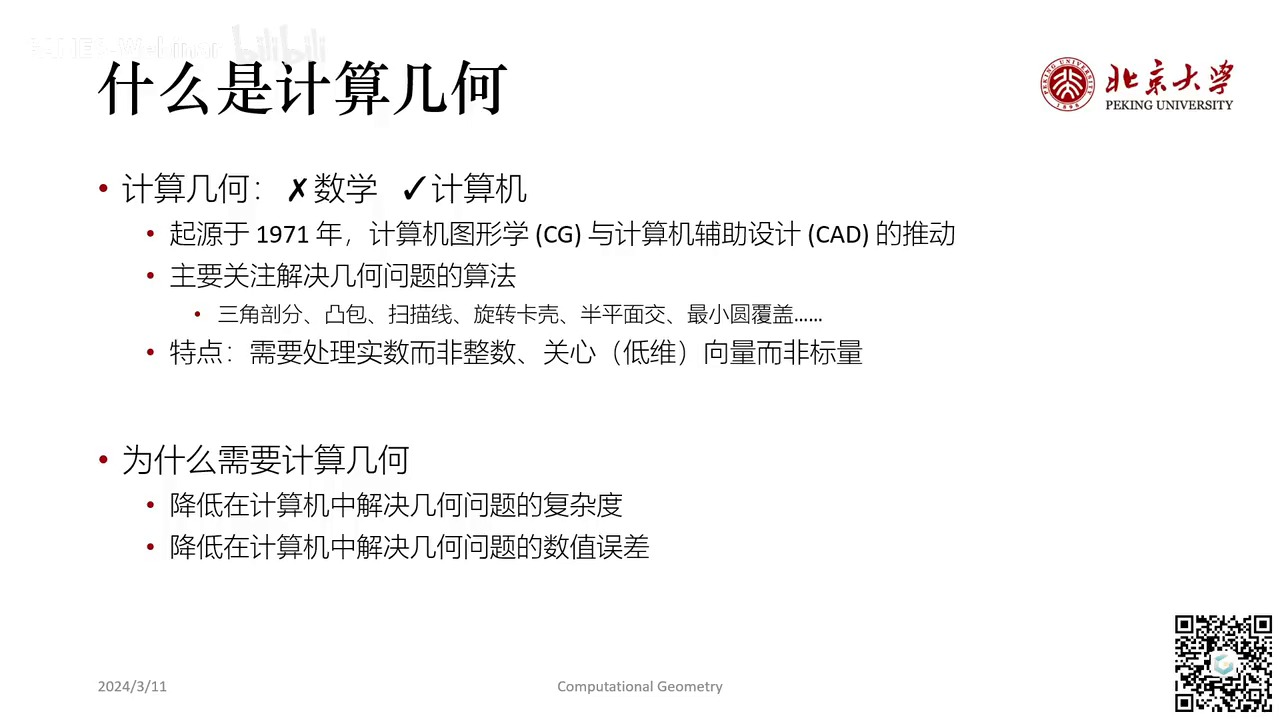
\includegraphics[width=0.92\textwidth]{figures/fig_01_intro_cg.jpg}
\caption{课件“什么是计算几何”：计算几何偏向计算机而非数学，关注几何问题的算法，特点是处理实数与低维向量\vtag}
\end{figure}
\srcnote{00:03:00--00:03:15}
\end{minipage}


\begin{importantbox}{本讲的主线}
本讲按“由简到繁”的顺序组织：先约定点、线、面的向量表示；再用点乘、叉乘计算距离、方向和相交关系；然后处理多边形的面积和包含关系、三角形之间的距离与碰撞检测；最后介绍德洛内三角剖分、凸包、平面最近点对、最小圆覆盖和反演变换几个经典算法。贯穿始终的思路是：\textbf{尽量用与维度无关的向量形式表达，尽量避免除法和三角函数}。
\end{importantbox}

\section{点、线、面的表示}

\subsection{坐标系的选取}

几何计算的第一步是选坐标系。我们希望基底是单位正交的，因为这样内积最好算；单位正交基底下的坐标就是笛卡尔坐标 $x,y,z$。原点的选取有任意性，但不同软件对“哪根轴竖直向上”和“左手系还是右手系”有不同约定，讲者把常见的四种列了出来：

\begin{itemize}
\item $y$ 轴竖直、右手系：Houdini、Maya。$x$ 指向屏幕右侧，$y$ 指向屏幕上方，$z$ 垂直屏幕朝外。
\item $y$ 轴竖直、左手系：Cinema4D、Unity3D、ZBrush、LightWave3D。$z$ 垂直屏幕朝内。
\item $z$ 轴竖直、右手系：Blender、3DSMax、CryEngine、SketchUp。$y$ 垂直屏幕朝内。
\item $z$ 轴竖直、左手系：Unreal。
\end{itemize}

此外，OpenGL 使用右手系，Direct3D 使用左手系。在不同软件之间导入导出模型时，坐标系不一致是最常见的错误来源之一。

\noindent\begin{minipage}{\textwidth}
\begin{figure}[H]
\centering
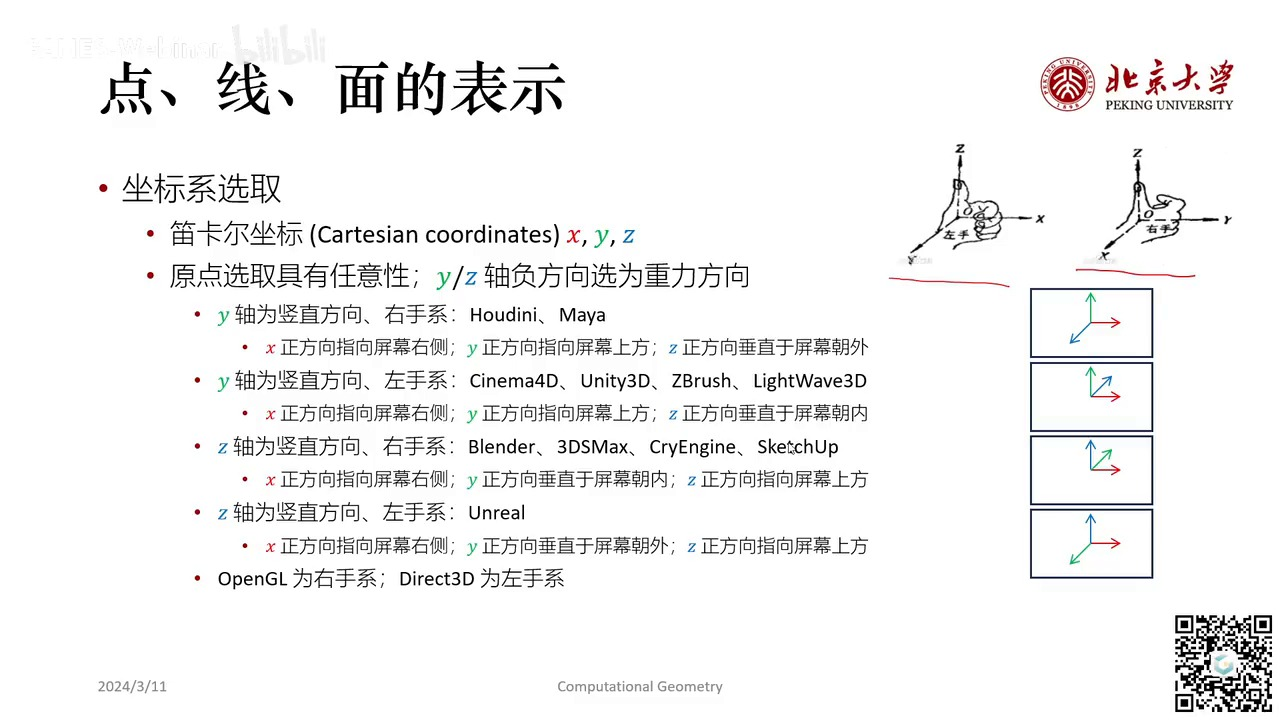
\includegraphics[width=0.92\textwidth]{figures/fig_02_coord_systems.jpg}
\caption{四种常见坐标系约定及对应软件；右上角是用左右手判断坐标系取向的示意\vtag}
\end{figure}
\srcnote{00:08:00--00:08:15}
\end{minipage}


\begin{knowledgebox}{如何用手判断左手系与右手系}
讲者介绍了两种用手判断坐标系取向的办法。一种是伸出拇指、食指和中指互相垂直，分别对应 $x,y,z$；另一种是四指从 $x$ 弯向 $y$，拇指指向 $z$。哪只手能做到，就是哪种坐标系。他更推荐第二种，因为它和叉乘 $\mathbf x\times\mathbf y=\mathbf z$ 的方向规则是一致的。
\end{knowledgebox}

\subsection{点与线}

确定坐标系后，点一般等同于向量：它可以看成从原点到该点的位置矢量（position vector），在二维或三维单位正交基底下用坐标表示。程序里也可以把点和向量区分开，即 \texttt{class Point} 与 \texttt{class Vector} 不同。这样做的好处是能让类型系统挡住无意义的运算：
\[
\text{Point}-\text{Point}\to\text{Vector},\qquad
\text{Point}\pm\text{Vector}\to\text{Point},\qquad
\text{Point}+\text{Point}\to\text{undefined}.
\]

直线和射线都可以写成“从点 $\mathbf p$ 出发、沿方向 $\mathbf v$ 前进”的参数方程：
\[
\mathbf x(t)=\mathbf p+t\mathbf v,\qquad t\in(-\infty,+\infty)\ \text{（直线）}\quad\text{或}\quad t\in[0,+\infty)\ \text{（射线）}.
\]
线段由两个端点 $\mathbf p_1,\mathbf p_2$ 给出：
\[
\mathbf x(t)=\mathbf p_1+t(\mathbf p_2-\mathbf p_1)=(1-t)\mathbf p_1+t\mathbf p_2,\qquad t\in[0,1].
\]
这些表达对二维和三维都成立。

\noindent\begin{minipage}{\textwidth}
\begin{figure}[H]
\centering
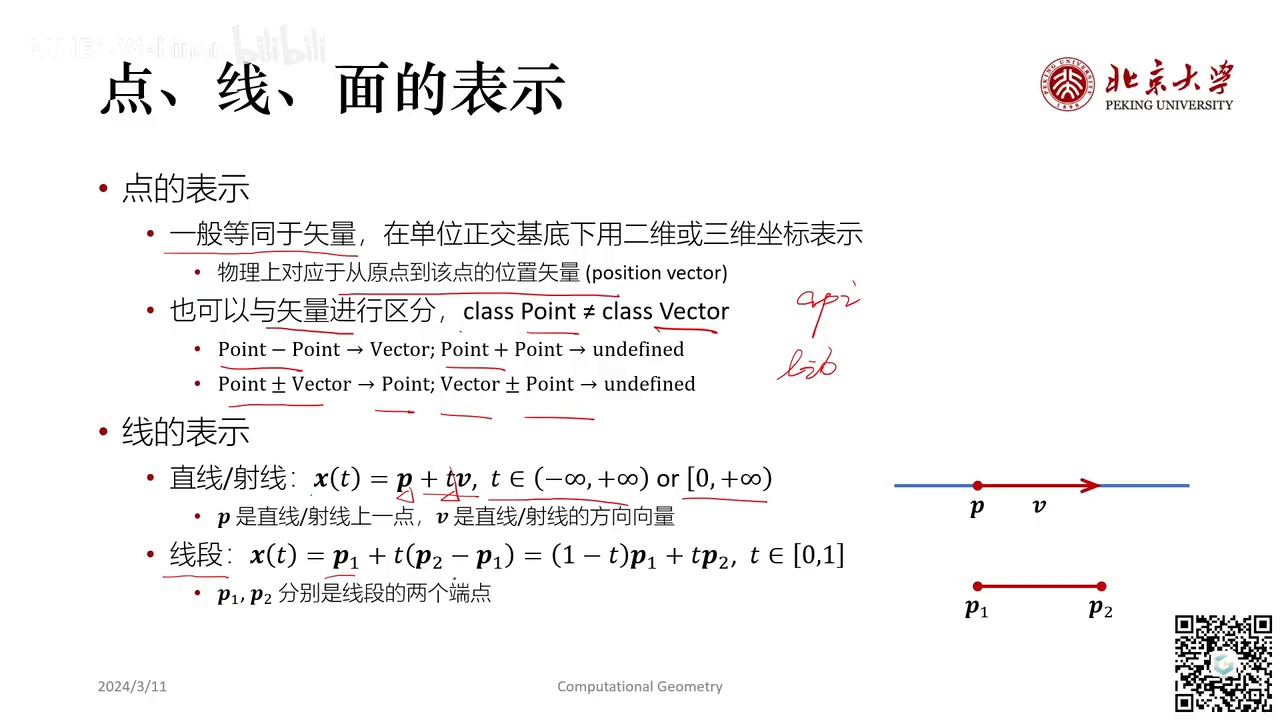
\includegraphics[width=0.92\textwidth]{figures/fig_03_point_line_repr.jpg}
\caption{点与线的表示：点等同于位置矢量；直线、射线、线段都用参数 $t$ 的取值范围区分\vtag}
\end{figure}
\srcnote{00:09:45--00:10:00}
\end{minipage}


\subsection{平面、半平面与三角形}

面是三维中的概念。无穷大的平面可以用隐式方程表示，其中 $\mathbf p$ 是平面上任意一点，$\mathbf n$ 是法向量：
\[
(\mathbf x-\mathbf p)\cdot\mathbf n=0 .
\]
如果把等号改为不等号，$(\mathbf x-\mathbf p)\cdot\mathbf n\le0$ 描述的就是平面以下的半个空间。“半平面”这个名字容易误导：它不是平面，而是一半的空间。此时法向量的正负有意义，因为把 $\mathbf n$ 取负号就指代另一半空间。

三角形 $\mathbf p_1\mathbf p_2\mathbf p_3$ 内的点可以用两个参数写成
\[
\mathbf x=\mathbf p_1+u(\mathbf p_2-\mathbf p_1)+v(\mathbf p_3-\mathbf p_1)=(1-u-v)\mathbf p_1+u\mathbf p_2+v\mathbf p_3 .
\]
为了把 $\mathbf x$ 限制在三角形内，可以分两步构造：先在 $\mathbf p_1,\mathbf p_2$ 之间取一点 $\mathbf x'=(1-t')\mathbf p_1+t'\mathbf p_2$，再在 $\mathbf x'$ 与 $\mathbf p_3$ 之间取一点
\[
\mathbf x=(1-t)\mathbf x'+t\mathbf p_3=(1-t)(1-t')\mathbf p_1+(1-t)t'\mathbf p_2+t\mathbf p_3 .
\]
令 $u=(1-t)(1-t')$，$v=(1-t)t'$，$w=t$，就得到
\[
\mathbf x=u\mathbf p_1+v\mathbf p_2+w\mathbf p_3,\qquad u+v+w=1,\quad u,v,w\ge0 .
\]
三个权重之和等于一，这就是重心坐标。后面计算点到三角形距离时还会用到它。

\noindent\begin{minipage}{\textwidth}
\begin{figure}[H]
\centering
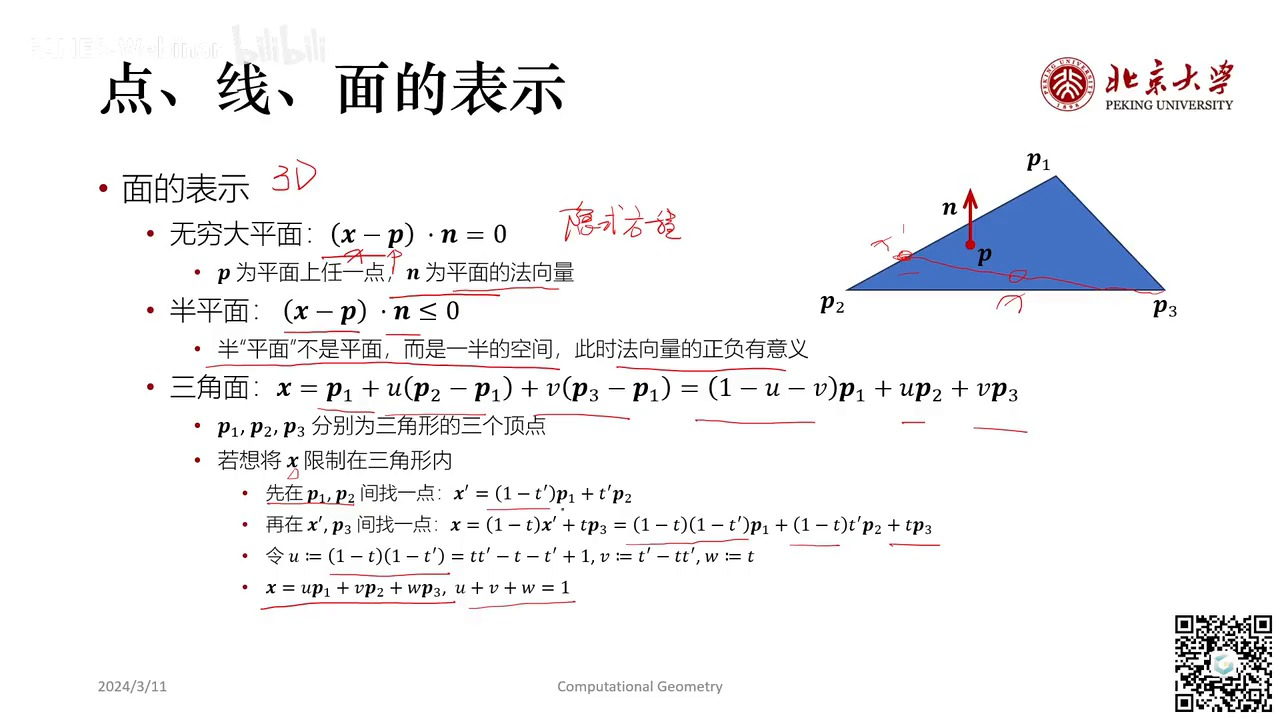
\includegraphics[width=0.92\textwidth]{figures/fig_04_plane_triangle.jpg}
\caption{面的表示：无穷大平面、半平面和三角形的参数表示，右侧为三角形 $\mathbf p_1\mathbf p_2\mathbf p_3$ 与法向量 $\mathbf n$\vtag}
\end{figure}
\srcnote{00:13:15--00:13:30}
\end{minipage}


\begin{warningbox}{约束条件不能漏}
三角形参数式中 $u,v,w\ge0$ 与 $u+v+w=1$ 缺一不可：只要求和为一，得到的是整个平面；再加上非负，才被限制在三角形内。同理，线段的 $t\in[0,1]$、射线的 $t\ge0$ 也是表示的一部分，计算距离时必须检查参数是否越界。
\end{warningbox}

\section{距离与位置关系：点乘和叉乘的组合}

讲者强调，之所以用向量而不是坐标展开来定义点和线，是因为向量形式算出来的距离公式\emph{与维度无关}：二维和三维可以用同一套代码。

\subsection{点与直线、射线的距离}

给定点 $\mathbf p$ 和直线 $\mathbf x=\mathbf o+t\mathbf d$。叉乘 $(\mathbf p-\mathbf o)\times\mathbf d$ 的模长是以这两个向量为边的平行四边形面积，即三角形面积的两倍；再除以底边长 $\|\mathbf d\|$，得到的正是三角形沿 $\mathbf d$ 这条边的高，也就是点到直线的距离：
\[
\mathrm{Dist}=h=\frac{\|(\mathbf p-\mathbf o)\times\mathbf d\|}{\|\mathbf d\|}.
\]

求点在直线上的投影 $\mathbf q=\mathbf o+t\mathbf d$ 时，利用 $\mathbf p-\mathbf q$ 与 $\mathbf d$ 垂直：
\[
(\mathbf o+t\mathbf d-\mathbf p)\cdot\mathbf d=0
\;\Longrightarrow\;
t=\frac{(\mathbf p-\mathbf o)\cdot\mathbf d}{\|\mathbf d\|^2},\qquad
\mathbf q=\mathbf o+\frac{(\mathbf p-\mathbf o)\cdot\mathbf d}{\|\mathbf d\|^2}\,\mathbf d .
\]

点到射线的距离也一样：先求 $t$。若 $t\ge0$，投影落在射线上，距离就是到直线的距离 $h$；若 $t<0$，投影落在射线端点的另一侧，最近点是端点本身，距离为 $\|\mathbf p-\mathbf o\|$。点到线段的距离同理，只需再检查 $t>1$ 的情况。

\noindent\begin{minipage}{\textwidth}
\begin{figure}[H]
\centering
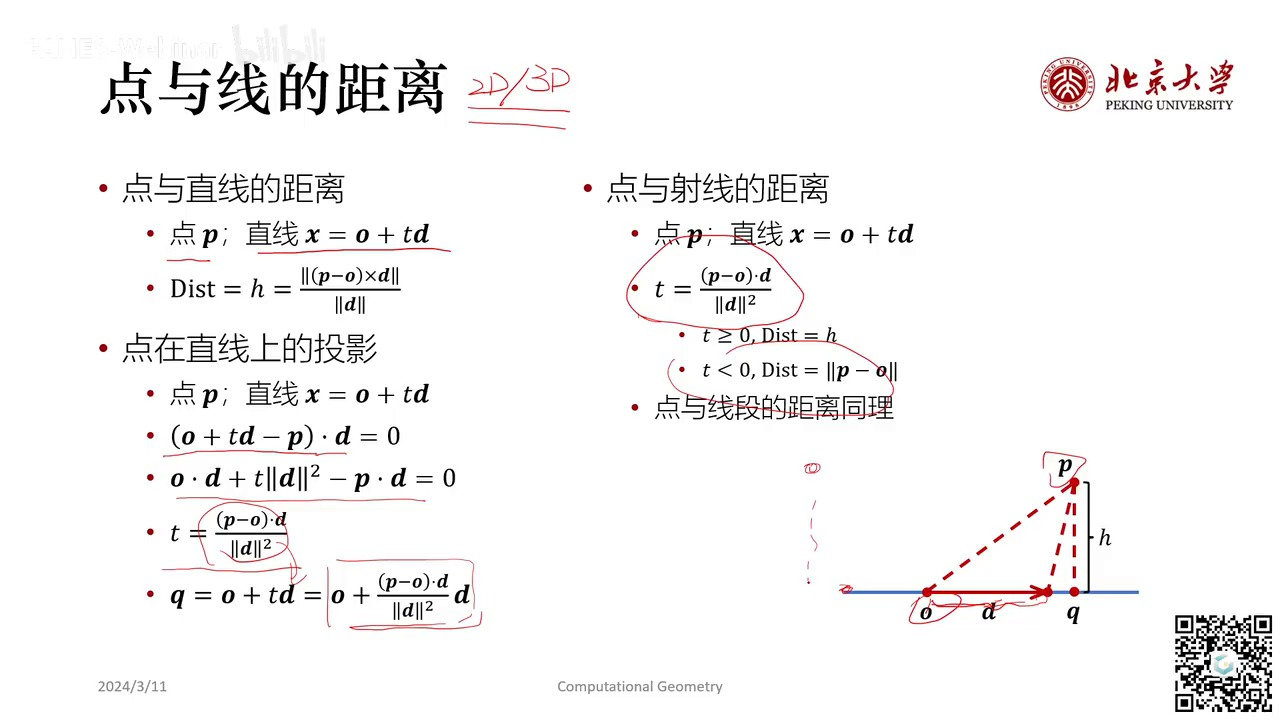
\includegraphics[width=0.92\textwidth]{figures/fig_05_point_line_dist.jpg}
\caption{点与直线、射线的距离：叉乘给出高 $h$，点乘给出投影参数 $t$\vtag}
\end{figure}
\srcnote{00:16:15--00:16:30}
\end{minipage}


\subsection{二维中线与线的方向关系}

设射线 1、2 有共同端点 $\mathbf o$，方向向量分别为 $\mathbf d_1=\mathbf p_1-\mathbf o$，$\mathbf d_2=\mathbf p_2-\mathbf o$。二维叉乘的结果是一个实数：
\[
\mathbf d_1\times\mathbf d_2=x_1y_2-x_2y_1 .
\]
它的符号给出了绕序：大于零，射线 2 在射线 1 的“左边”（逆时针转角小于 $180^\circ$）；小于零，射线 2 在射线 1 的“右边”（顺时针转角小于 $180^\circ$）；等于零，两射线重合或方向相反。最后一种情况还需要用点乘进一步判断：重合时点乘大于零，反向时点乘小于零。

\noindent\begin{minipage}{\textwidth}
\begin{figure}[H]
\centering
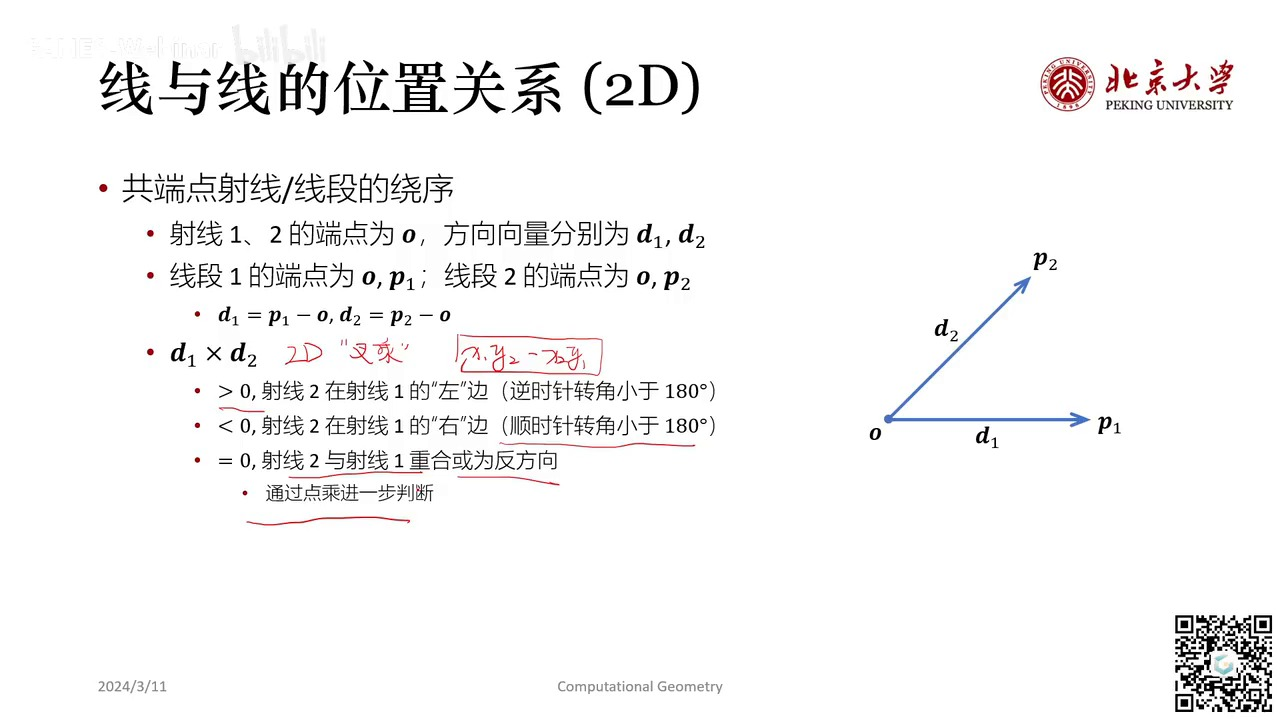
\includegraphics[width=0.92\textwidth]{figures/fig_06_orientation_2d.jpg}
\caption{共端点射线的绕序：用二维叉乘的符号判断“左边”和“右边”\vtag}
\end{figure}
\srcnote{00:18:00--00:18:15}
\end{minipage}


\begin{knowledgebox}{二维“叉乘”是什么}
严格地说叉乘只在三维中定义。二维中的 $x_1y_2-x_2y_1$ 可以看成把两个向量补上 $z=0$ 后做三维叉乘，取结果的 $z$ 分量；它也等于以两向量为列的 $2\times2$ 行列式，即有向面积。本讲中的大量判断，包括绕序、跨立测试、凸包和多边形面积，都建立在这个有向面积的符号上。
\end{knowledgebox}

\subsection{直线的交点与线段的跨立测试}

直线 1：$\mathbf x_1=\mathbf o_1+t_1\mathbf d_1$；直线 2：$\mathbf x_2=\mathbf o_2+t_2\mathbf d_2$。交点同时在两条直线上，所以直线 2 上的点减去 $\mathbf o_1$ 必须与 $\mathbf d_1$ 平行：
\[
[(\mathbf o_2+t_2\mathbf d_2)-\mathbf o_1]\times\mathbf d_1=0
\;\Longrightarrow\;
t_2=\frac{\mathbf d_1\times(\mathbf o_2-\mathbf o_1)}{\mathbf d_2\times\mathbf d_1},\qquad
\mathbf p=\mathbf o_2+t_2\mathbf d_2 .
\]
展开后这是关于 $t_2$ 的线性方程，直接解出即可。

判断两条\emph{线段}是否相交，可以不求交点，而用跨立测试。线段 1 的端点为 $\mathbf p_1,\mathbf q_1$，线段 2 的端点为 $\mathbf p_2,\mathbf q_2$，令
\[
\begin{gathered}
s_1=[(\mathbf q_1-\mathbf p_1)\times(\mathbf p_2-\mathbf p_1)]\cdot[(\mathbf q_1-\mathbf p_1)\times(\mathbf q_2-\mathbf p_1)],\\
s_2=[(\mathbf q_2-\mathbf p_2)\times(\mathbf p_1-\mathbf p_2)]\cdot[(\mathbf q_2-\mathbf p_2)\times(\mathbf q_1-\mathbf p_2)].
\end{gathered}
\]
$s_1\le0$ 的意思是：线段 2 的两个端点分别位于线段 1 所在直线的两侧（或在直线上）。两线段相交，当且仅当 $s_1\le0$ 且 $s_2\le0$；取等号时交点在端点处。

\noindent\begin{minipage}{\textwidth}
\begin{figure}[H]
\centering
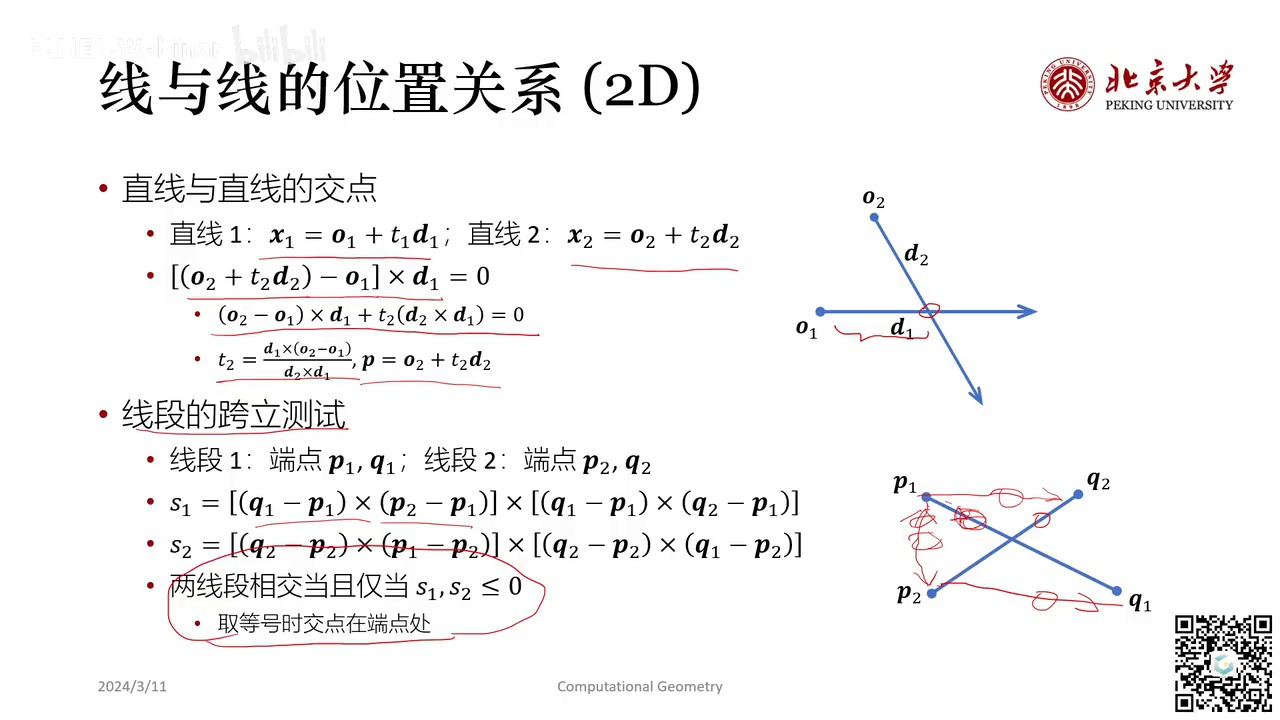
\includegraphics[width=0.92\textwidth]{figures/fig_07_line_intersect.jpg}
\caption{直线与直线的交点，以及线段的跨立测试 $s_1,s_2\le0$\vtag}
\end{figure}
\srcnote{00:21:15--00:21:30}
\end{minipage}


\begin{importantbox}{跨立测试为什么好}
跨立测试只用了减法、乘法和比较，\textbf{没有做任何除法}。除法会放大误差，还要单独处理分母为零（平行）的情况。几何谓词能不除就不除，这是计算几何控制数值误差最朴素也最有效的手段。
\end{importantbox}

\subsection{三维中异面直线的距离}

三维中两条直线 $\mathbf x_1=\mathbf o_1+t_1\mathbf d_1$ 和 $\mathbf x_2=\mathbf o_2+t_2\mathbf d_2$ 一般不相交，而是异面。讲者给了两种求距离的方法。

方法一：求两直线的公垂线方向，再把连接两直线上任意两点的向量投影到这个方向上：
\[
\mathbf n=\frac{\mathbf d_1\times\mathbf d_2}{\|\mathbf d_1\times\mathbf d_2\|},\qquad
\mathrm{Dist}=|\mathbf n\cdot(\mathbf o_2-\mathbf o_1)| .
\]

方法二：联立方程求极值。把两直线上点的距离写成两个参数的函数
\[
\|\mathbf x_2-\mathbf x_1\|=\|\mathbf o_2+t_2\mathbf d_2-\mathbf o_1-t_1\mathbf d_1\|,
\]
对 $t_1,t_2$ 分别求偏导并令其为零。

知道异面直线的距离后，异面\emph{线段}的距离也可以处理：把它们投影到同一平面上做跨立测试，或者把参数约束在 $[0,1]$ 内，当作带约束的优化问题求极值。

\noindent\begin{minipage}{\textwidth}
\begin{figure}[H]
\centering
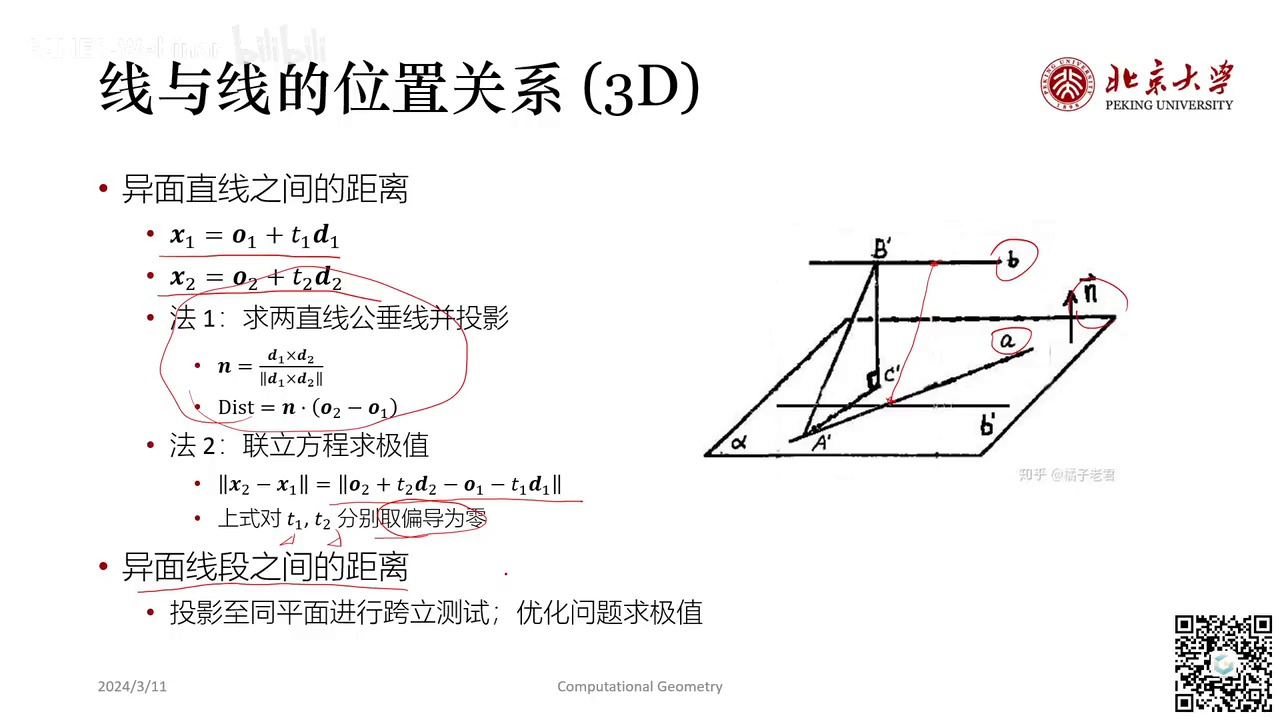
\includegraphics[width=0.92\textwidth]{figures/fig_08_skew_lines.jpg}
\caption{异面直线之间的距离：公垂线投影法与联立求极值法\vtag}
\end{figure}
\srcnote{00:23:30--00:23:45}
\end{minipage}


\subsection{点与面的距离}

平面 $(\mathbf x-\mathbf p)\cdot\mathbf n=0$ 外有一点 $\mathbf x$。在平面上任取一点 $\mathbf p$，把 $\mathbf x-\mathbf p$ 投影到法向量上，就得到距离：
\[
\mathrm{Dist}=\frac{|(\mathbf x-\mathbf p)\cdot\mathbf n|}{\|\mathbf n\|}.
\]
这个距离不受 $\mathbf p$ 选取的影响。原因是：换成平面上另一点 $\mathbf p'$，差 $\mathbf p'-\mathbf p$ 位于平面内，与 $\mathbf n$ 点乘后消掉。

把向量形式展开，$(x-p_x,y-p_y,z-p_z)\cdot(n_x,n_y,n_z)=0$ 就整理成高等数学课上熟悉的 $Ax+By+Cz+D=0$，距离公式也与 $|Ax+By+Cz+D|/\sqrt{A^2+B^2+C^2}$ 完全一致。讲者在手写板上补充：二维中点到直线 $Ax+By+C=0$ 的距离也是同一个式子去掉 $z$ 项。

\noindent\begin{minipage}{\textwidth}
\begin{figure}[H]
\centering
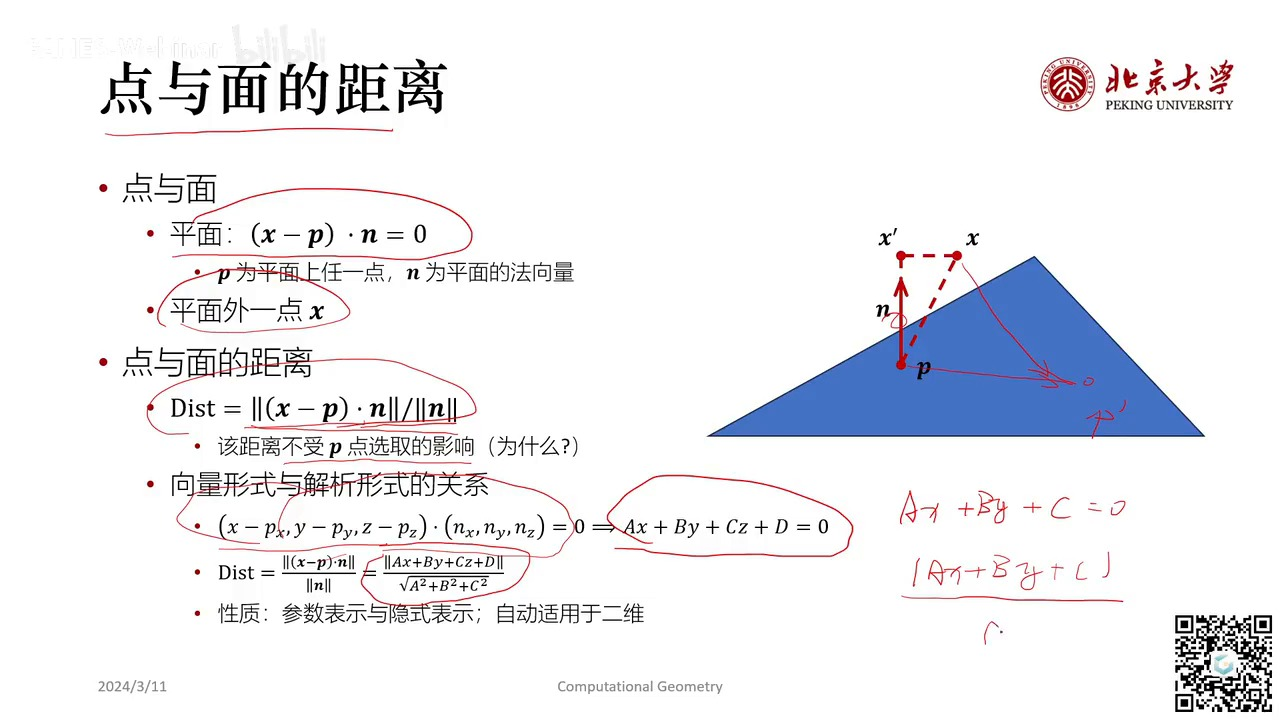
\includegraphics[width=0.92\textwidth]{figures/fig_09_point_plane_hand.jpg}
\caption{点与面的距离：向量形式与解析形式一致，手写补充二维点到直线的同型公式\vtag}
\end{figure}
\srcnote{00:26:45--00:27:00}
\end{minipage}


\begin{knowledgebox}{为什么偏爱向量形式}
既然解析式和向量式算出来一样，为什么计算几何更爱用向量式？讲者给出两点理由。其一，向量式自动适用于二维和三维：同一个 $\|(\mathbf x-\mathbf p)\cdot\mathbf n\|/\|\mathbf n\|$ 既能求二维中点到线的距离，也能求三维中点到面的距离。其二，它连接了参数表示与隐式表示：直线只要取方向向量就能参数化；平面若要参数化，还需要先取两个切向量来搭建平面内的坐标轴，而隐式式只需要一个法向量。
\end{knowledgebox}

\section{多边形：周长、面积与包含关系}

\subsection{周长与面积}

多边形的周长最好算：遍历每条边，把模长相加即可。面积要借助叉乘。假定多边形按逆时针顺序给出顶点。三角形的面积是
\[
A_{123}=\tfrac12\|(\mathbf p_2-\mathbf p_1)\times(\mathbf p_3-\mathbf p_1)\| .
\]
如果去掉绝对值、保留符号，得到有向面积。在平面上任取一点 $\mathbf p_0$，则
\[
A_{123}=A_{012}+A_{023}-A_{013}=A_{012}+A_{023}+A_{031},
\]
因为把 $A_{013}$ 的绕序反过来就是 $A_{031}$，符号也随之反号。对凸多边形，$A_{1234}=A_{123}+A_{134}$；对任意多边形，同样可以取任意参考点 $\mathbf p_0$：
\[
A_{1234}=A_{012}+A_{023}+A_{034}+A_{041},\qquad
A=\sum_{i=1,\ j=(i\bmod n)+1}^{n}A_{0ij}.
\]

\noindent\begin{minipage}{\textwidth}
\begin{figure}[H]
\centering
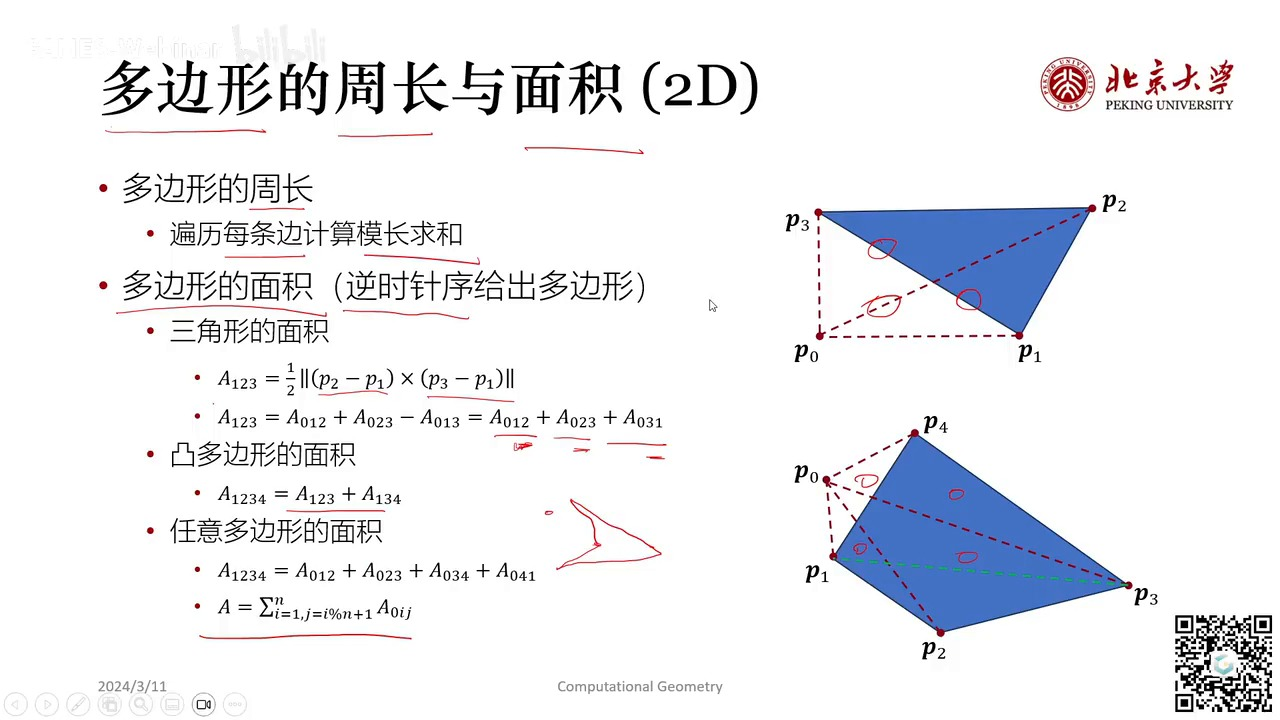
\includegraphics[width=0.92\textwidth]{figures/fig_10_polygon_area.jpg}
\caption{多边形面积：以任意点 $\mathbf p_0$ 为参考，按逆时针绕序累加有向三角形面积\vtag}
\end{figure}
\srcnote{00:33:00--00:33:15}
\end{minipage}


\begin{importantbox}{有向面积让凹多边形也能算}
用一个外部参考点把多边形拆成扇形三角形，凸多边形和凹多边形都适用。关键在于“有向”：参考点在多边形外时，一部分三角形的面积为负，正好抵消多算的部分。若取绝对值，结果就错了。
\end{importantbox}

\subsection{点与凸多边形的位置关系}

判断点 $\mathbf p_0$ 是否在凸多边形内，有两种方法。

\textbf{面积法}。按逆时针顺序给出多边形，分别计算带符号和带绝对值的面积：
\[
A=\sum_{i=0}^{n-1}A_{0ij},\qquad
A'=\sum_{i=0}^{n-1}|A_{0ij}|,\qquad j=(i+1)\bmod n .
\]
若 $A$ 与 $A'$ 相等，则 $\mathbf p_0$ 在多边形内。参考点在内部时，每个三角形都是正向的；参考点在外部时，必有部分三角形为负，绝对值求和就比带符号求和大。

\textbf{绕序法}。逐边检查 $\mathbf p_0$ 是否在每一条边的“左边”：
\[
(\mathbf p_i-\mathbf p_0)\times(\mathbf p_{i+1}-\mathbf p_0)>0\quad\text{对所有 } i\ \text{成立} .
\]
只要有一条边不满足，点就不在凸多边形内。讲者留了一个思考题：上述判断很容易推广到三维，把面积换成体积，把边换成面，就得到点与凸多面体的位置关系。

\noindent\begin{minipage}{\textwidth}
\begin{figure}[H]
\centering
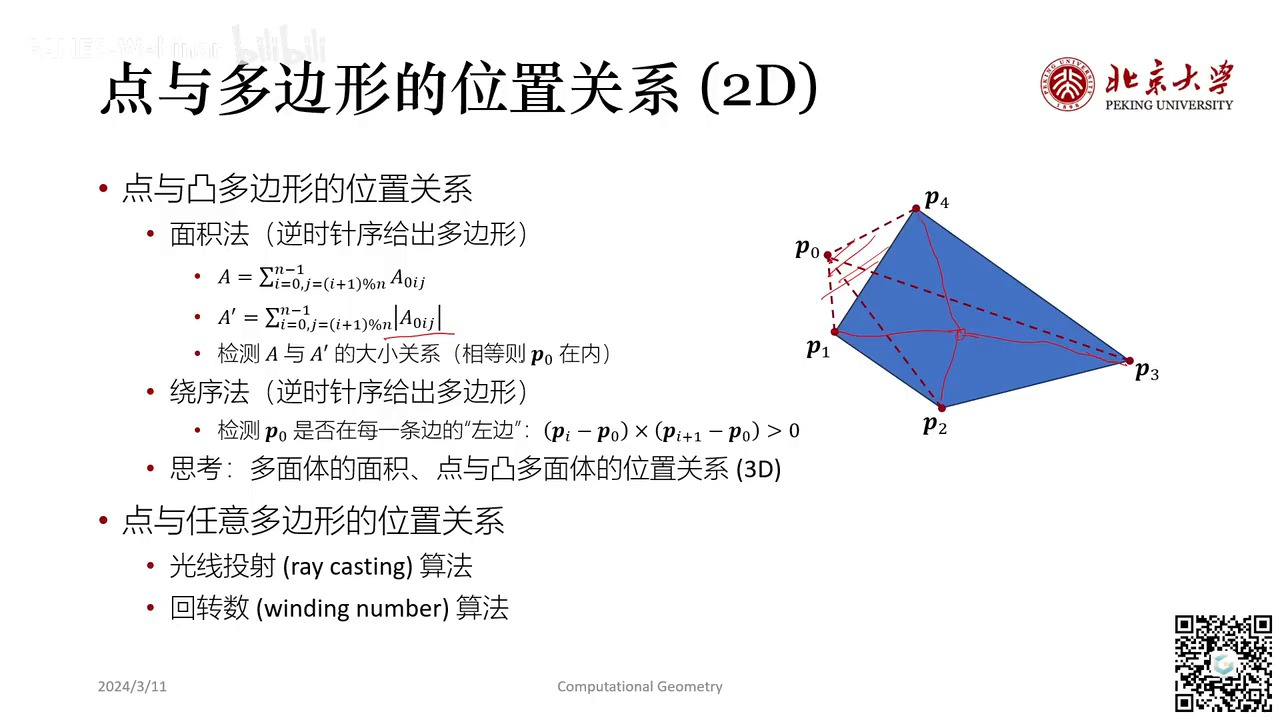
\includegraphics[width=0.92\textwidth]{figures/fig_11_point_convex_polygon.jpg}
\caption{点与凸多边形的位置关系：面积法与绕序法\vtag}
\end{figure}
\srcnote{00:34:15--00:34:30}
\end{minipage}


\subsection{点与任意多边形：光线投射法}

对任意（可能是凹的）多边形，上面的方法不再成立，需要用到若尔当（Jordan）曲线定理：任意一条简单闭曲线把平面分成内、外两部分。连接同一部分中任意两点的弧，与该曲线不相交或相交偶数次；连接不同部分两点的弧，与该曲线相交奇数次。

多边形是简单闭曲线。从待判断点向无穷远发出一条射线，就把射线当作定理中的弧。弧每与多边形相交一次，内外关系就改变一次，而无穷远点一定在多边形外，因为多边形是有限的。于是：相交次数为奇数，点在多边形内；相交次数为偶数，点在多边形外。

\noindent\begin{minipage}{\textwidth}
\begin{figure}[H]
\centering
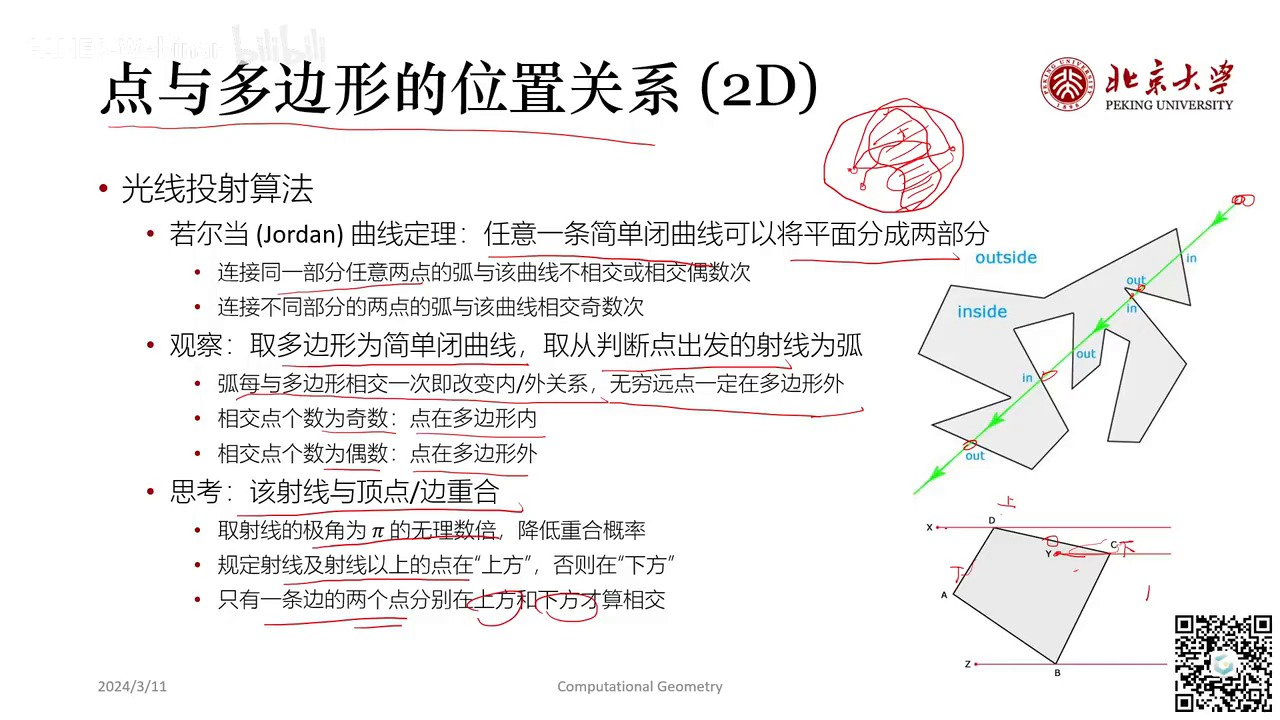
\includegraphics[width=0.92\textwidth]{figures/fig_12_ray_casting.jpg}
\caption{光线投射法：从点出发的射线与多边形边界相交次数的奇偶决定内外；手写示意射线经过顶点的特殊情况\vtag}
\end{figure}
\srcnote{00:42:00--00:42:15}
\end{minipage}


\begin{warningbox}{射线与顶点、边重合}
射线恰好经过多边形顶点或与边重合时，交点会被重复计数或漏计。讲者给了两个对策。一是让射线的极角取一个与 $\pi$ 无理相关的数，大大降低重合的概率。二是规定射线及其以上的点都算“上方”、以下的点算“下方”，只有一条边的两个端点分别在上方和下方时才算相交。用第二个规则判断课件中的四边形时，与边 $CD$ 重合的情况因为 $C,D$ 都在“上方”而不计数，从而避开了数值上的歧义。
\end{warningbox}

\subsection{回转数算法}

另一种方法是回转数（winding number），即曲线绕过一点的次数。对多边形内的点，逆时针给出的多边形绕它一次，回转数为 1；对多边形外的点，绕它的次数为 0。回转数等于回转角 $\theta$ 除以 $2\pi$，而回转角可以把每条边对该点张成的有向角相加：
\[
\theta=\sum_{i=1,\ j=(i\bmod n)+1}^{n}\arcsin\frac{\|(\mathbf p_i-\mathbf p_0)\times(\mathbf p_j-\mathbf p_0)\|}{\|\mathbf p_i-\mathbf p_0\|\,\|\mathbf p_j-\mathbf p_0\|} .
\]
这里叉乘取带符号的值，逆时针为正、顺时针为负。对于自交曲线，回转数可以是 $-2,-1,0,1,2,3,\dots$，绝对值大于一的情况说明曲线绕了该点不止一圈。

\noindent\begin{minipage}{\textwidth}
\begin{figure}[H]
\centering
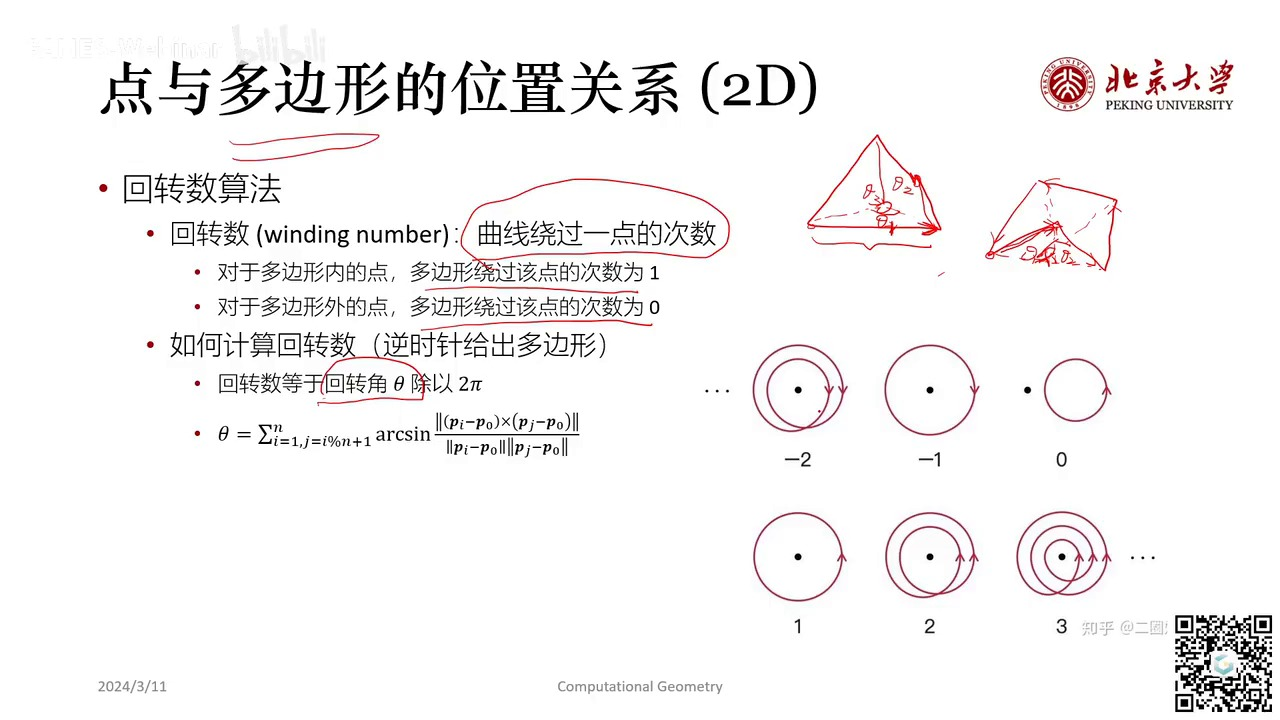
\includegraphics[width=0.92\textwidth]{figures/fig_13_winding.jpg}
\caption{回转数：曲线绕过一点的圈数，课件右下给出 $-2$ 到 $3$ 的例子\vtag}
\end{figure}
\srcnote{00:45:15--00:45:30}
\end{minipage}


\begin{warningbox}{$\arcsin$ 只给出 $[-\pi/2,\pi/2]$}
课件上的式子用 $\arcsin$ 表示每条边张成的角。讲义作者补充：$\arcsin$ 的值域只有 $[-\pi/2,\pi/2]$，当某条边对该点的张角超过 $90^\circ$ 时会算错。实现时通常用 $\operatorname{atan2}(\text{叉乘},\text{点乘})$ 求有向角，值域是 $(-\pi,\pi]$，不会出现这个问题。
\end{warningbox}

\section{三角形之间的距离与碰撞检测}

\subsection{点到三角形的距离}

在图形学中，网格（mesh）由一个个面（face）组成，求点到网格的距离就要对每个面求点到三角形的距离，再取最小值。讲者因此说，这是计算几何在 CG 中最重要的应用之一。

\textbf{二维情形}。点在三角形内，距离为零。点在三角形外时，先令 Dist 为点到三个顶点距离的最小值；再把点分别投影到三条边所在的直线上，若投影点落在边上（而不是延长线上），就用点到边的距离更新 Dist。

\textbf{三维情形}。先把点投影到三角形所在的平面，记投影距离为 $D_1$；再在平面内按二维方法求投影点到三角形的距离 $D_2$。由勾股定理，
\[
D=\sqrt{D_1^2+D_2^2}.
\]

\textbf{其它方法}。利用三角形的参数表示，三角形上任一点为 $\mathbf p=u\mathbf p_1+v\mathbf p_2+w\mathbf p_3$，约束为 $u+v+w=1$ 且 $u,v,w\ge0$。把它与三角形外的点作差、求模长平方，就变成一个带约束的二次优化问题。

\noindent\begin{minipage}{\textwidth}
\begin{figure}[H]
\centering
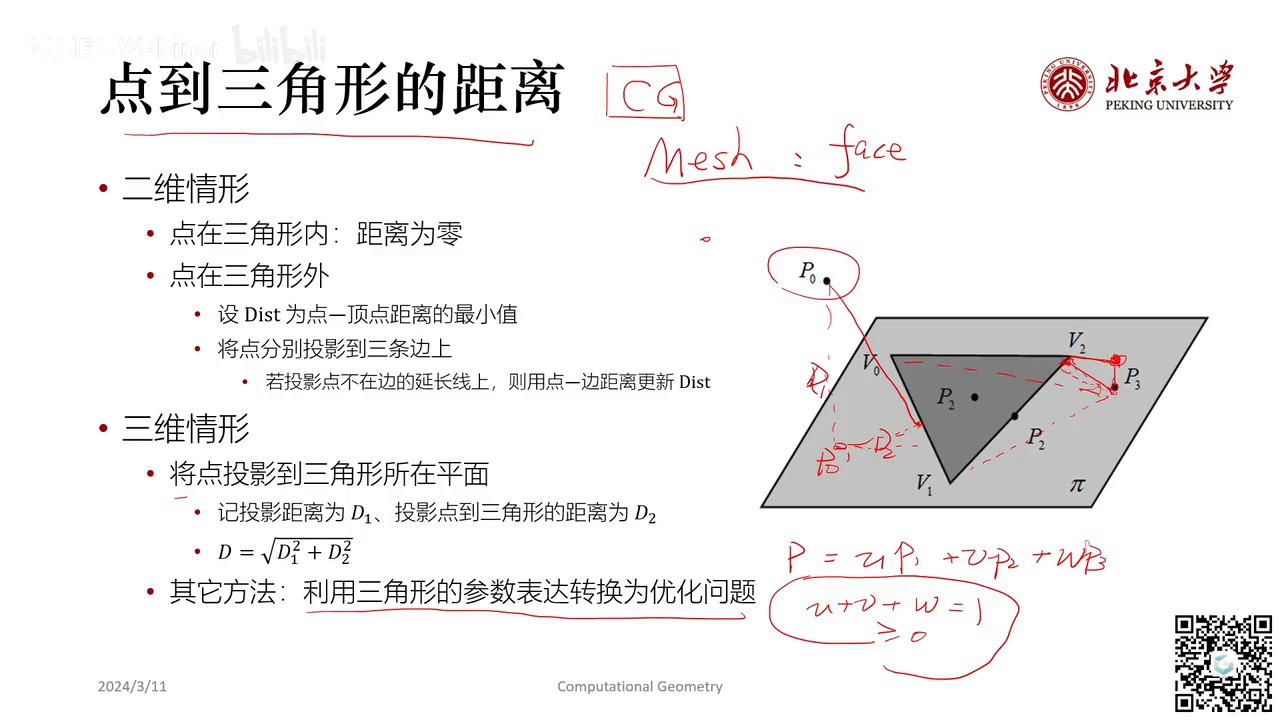
\includegraphics[width=0.92\textwidth]{figures/fig_14_point_triangle.jpg}
\caption{点到三角形的距离：二维逐边投影，三维先投影到平面再用勾股定理；手写补充参数化优化\vtag}
\end{figure}
\srcnote{00:49:30--00:49:45}
\end{minipage}


\subsection{三角形之间的距离}

设两个三角形不相交。在\textbf{二维}中，最近距离一定在“一个三角形的顶点”与“另一个三角形”之间取到，所以只需比较 6 组点—面距离，即每个三角形的 3 个顶点到另一个三角形的距离；也可以比较 18 组点—边距离，即 6 个顶点乘以对方的 3 条边，取最小值。在二维中这是完备的。

在\textbf{三维}中仅有 6 组点—面距离不够：两个三角形的最近点可能出现在两条边的内部，比如两条交叉的边。因此还要加上 9 组边—边距离（$3\times3$），取全部 15 组中的最小值。

\noindent\begin{minipage}{\textwidth}
\begin{figure}[H]
\centering
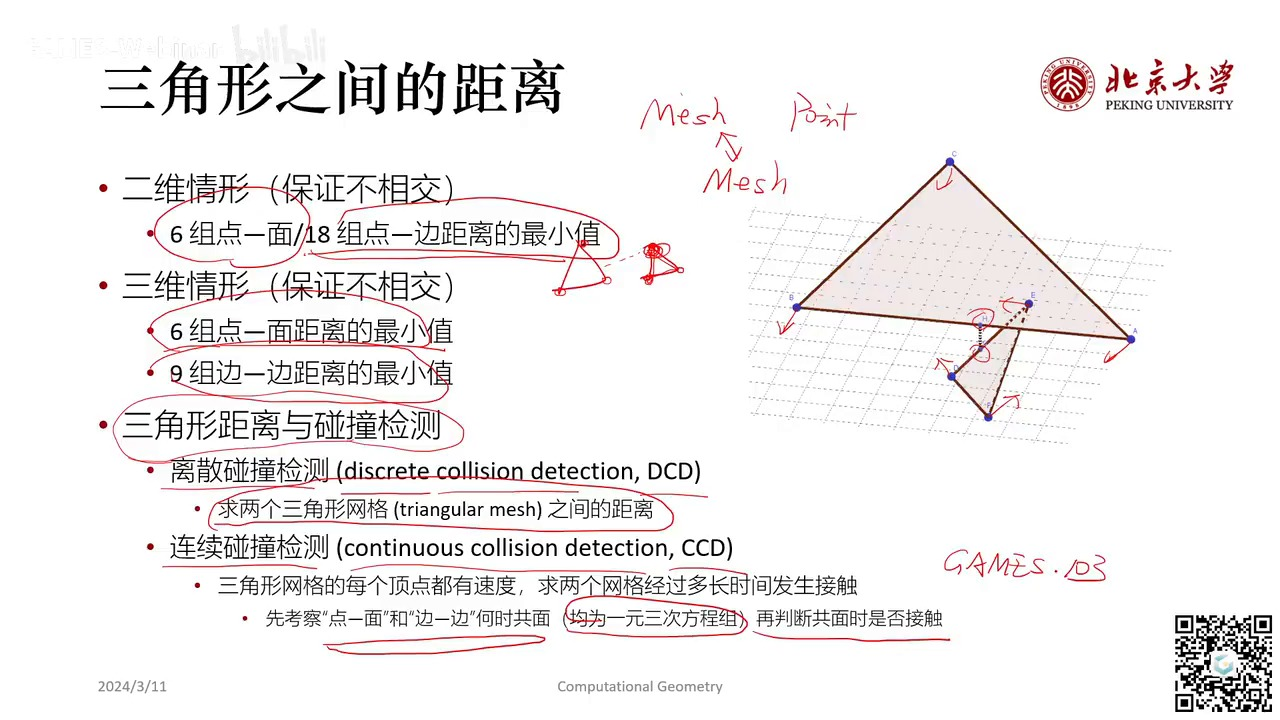
\includegraphics[width=0.92\textwidth]{figures/fig_15_tri_tri.jpg}
\caption{三角形之间的距离：二维 6 组点—面或 18 组点—边，三维 6 组点—面加 9 组边—边\vtag}
\end{figure}
\srcnote{00:54:15--00:54:30}
\end{minipage}


\subsection{离散与连续碰撞检测}

三角形距离直接服务于碰撞检测，图形学中一般分两类。

\begin{itemize}
\item \textbf{离散碰撞检测}（discrete collision detection, DCD）：在某一时刻求两个三角形网格之间的距离，判断是否已经接触或穿透。
\item \textbf{连续碰撞检测}（continuous collision detection, CCD）：网格的每个顶点都有速度，求两个网格经过多长时间发生接触。做法是先考察“点—面”和“边—边”两类图元何时共面，这两类共面条件都对应关于时间 $t$ 的一元三次方程；解出 $t$ 后，再判断共面时是否真正接触。
\end{itemize}

讲者提醒，CCD 在实现上相当困难，感兴趣的同学可以参考王华民老师 GAMES103 的第 9 讲。

\begin{knowledgebox}{CCD 中的三次方程从哪里来}
讲义作者补充：以点—面为例，点 $\mathbf x_0$ 与三角形顶点 $\mathbf x_1,\mathbf x_2,\mathbf x_3$ 都以匀速运动，$\mathbf x_i(t)=\mathbf x_i+t\mathbf v_i$。四点共面等价于
\[
\bigl[(\mathbf x_1(t)-\mathbf x_0(t))\times(\mathbf x_2(t)-\mathbf x_0(t))\bigr]\cdot(\mathbf x_3(t)-\mathbf x_0(t))=0 .
\]
三个因子各是 $t$ 的一次式，乘积是 $t$ 的三次多项式。边—边的情形完全类似。
\end{knowledgebox}

\section{德洛内三角剖分与沃罗诺伊图}

三角剖分把点集连接成三角网格，使得各三角形的边互不相交。德洛内（Delaunay）三角剖分是其中最常用的一种，它有两个等价的刻画：

\begin{itemize}
\item \textbf{空圆性}：任意三角形的外接圆内都没有其它点。
\item \textbf{规则化}：在所有三角剖分中，它使三角形的最小角最大，避免了狭长的“病态”三角形。
\end{itemize}

它还有几条性质：在点集一般位置（无四点共圆）时，所得结果唯一；增、删、改顶点只影响局部；最外层边界形成凸多边形，即点集的凸包。

德洛内三角剖分的对偶图是沃罗诺伊（Voronoi）图。它把平面划分成若干区域，每个区域由离它最近的控制点决定。构造方法是在三角剖分的每一条边上取中垂线，这些中垂线自然相交，交点正是各三角形外接圆的圆心，围成的格子就是沃罗诺伊图。

\noindent\begin{minipage}{\textwidth}
\begin{figure}[H]
\centering
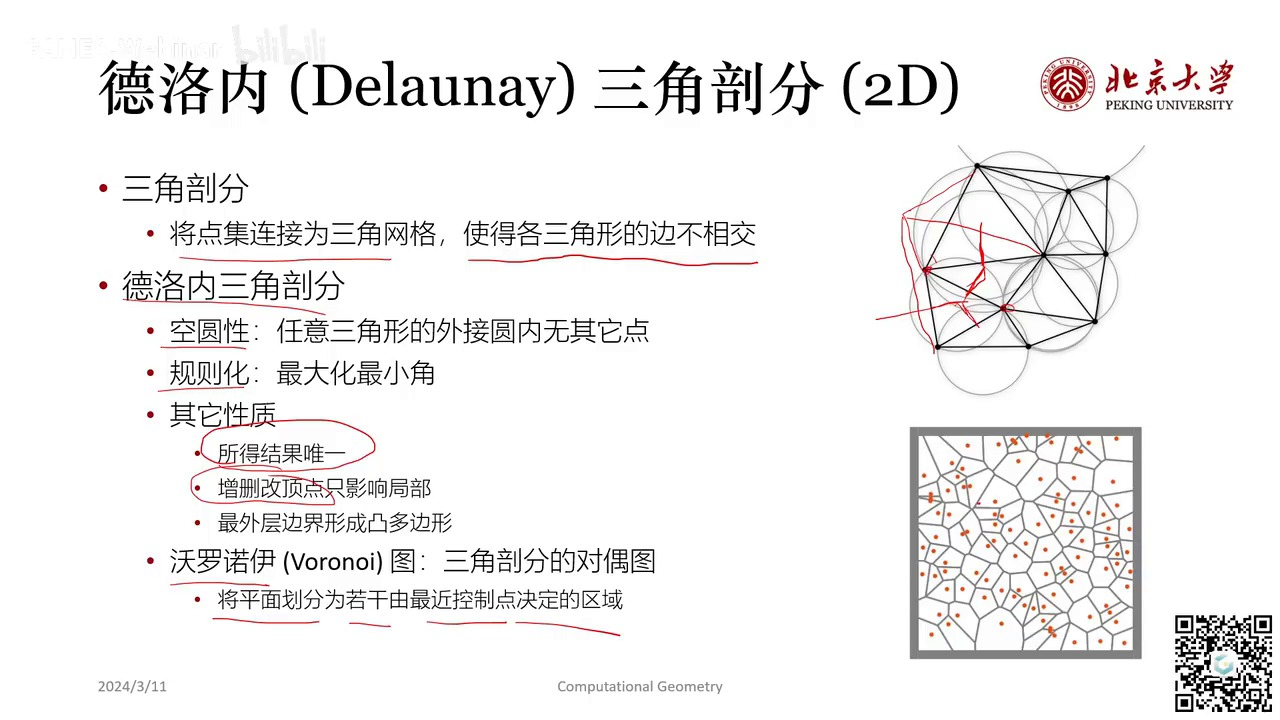
\includegraphics[width=0.92\textwidth]{figures/fig_16_delaunay.jpg}
\caption{德洛内三角剖分的空圆性（上）与对偶的沃罗诺伊图（下）\vtag}
\end{figure}
\srcnote{00:57:15--00:57:30}
\end{minipage}


\section{凸包}

\subsection{凸包与包围盒}

凸包是平面上包含给定点的最小凸多边形；凸多边形是所有内角都小于 $180^\circ$ 的多边形。图形学中经常使用比凸包更宽松、但更容易计算的包围结构：

\begin{itemize}
\item \textbf{轴对齐包围盒}（axis aligned bounding box, AABB）：包含给定点、边与坐标轴平行的矩形。凸包一定在 AABB 内，AABB 是凸包最粗糙的近似。
\item \textbf{方向包围盒}（oriented bounding box, OBB）：包含给定点的最小矩形，放宽了“与轴对齐”的限制，矩形可以倾斜。
\item \textbf{固定方向凸包}（fixed directions hulls, FDH）：“凸包”各边（面）的法向只能在给定的集合中选取。例如允许 $45^\circ$ 斜边，拼出的就是八边形。方向越多，越接近真正的凸包。
\end{itemize}

\noindent\begin{minipage}{\textwidth}
\begin{figure}[H]
\centering
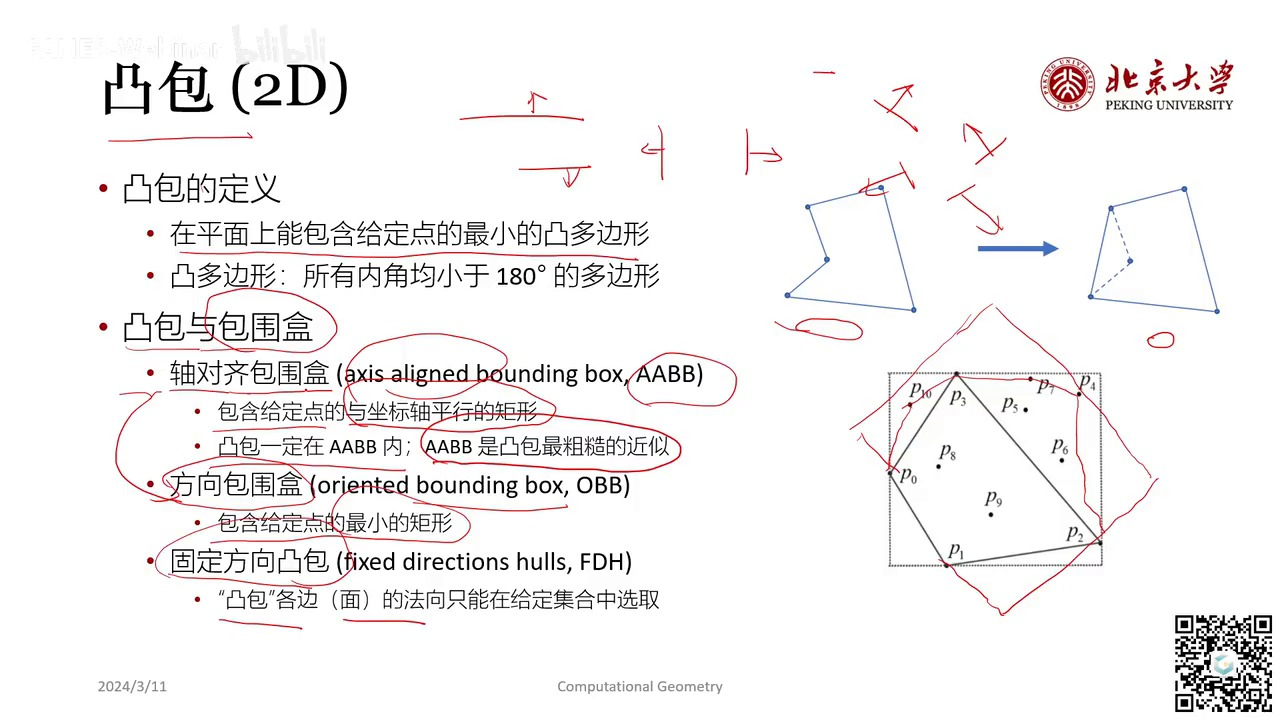
\includegraphics[width=0.92\textwidth]{figures/fig_17_bounding_boxes.jpg}
\caption{凸包的定义及其近似：AABB、OBB 与固定方向凸包\vtag}
\end{figure}
\srcnote{01:00:15--01:00:30}
\end{minipage}


\subsection{二维凸包：葛立恒扫描法}

葛立恒（Graham）扫描法基于两个观察。观察 1：点集中纵坐标最小的点一定在凸包上。观察 2：沿凸包逆时针走，经过的每一处都是“左拐”，这其实就是凸多边形内角小于 $180^\circ$ 的定义。算法流程如下：

\begin{enumerate}
\item 取点集中纵坐标最小的点 $\mathbf p_0$。
\item 以 $\mathbf p_0$ 为原点，把其余所有点按极角排序。
\item 维护一个栈，将 $\mathbf p_0,\mathbf p_1$ 压入。
\item 按极角顺序依次考察 $\mathbf p_2,\mathbf p_3,\dots$：设当前考察 $\mathbf p_i$，栈顶为 $\mathbf p_t$，栈顶下方为 $\mathbf p_s$。若
\[
(\mathbf p_t-\mathbf p_s)\times(\mathbf p_i-\mathbf p_t)>0,
\]
即 $\mathbf p_s\to\mathbf p_t\to\mathbf p_i$ 左拐，则把 $\mathbf p_i$ 压入栈中；否则弹出栈顶，重复判断。
\end{enumerate}

遍历完所有点后，栈中就是凸包。主要的时间代价在极角排序，时间复杂度为 $O(n\log n)$。

\noindent\begin{minipage}{\textwidth}
\begin{figure}[H]
\centering
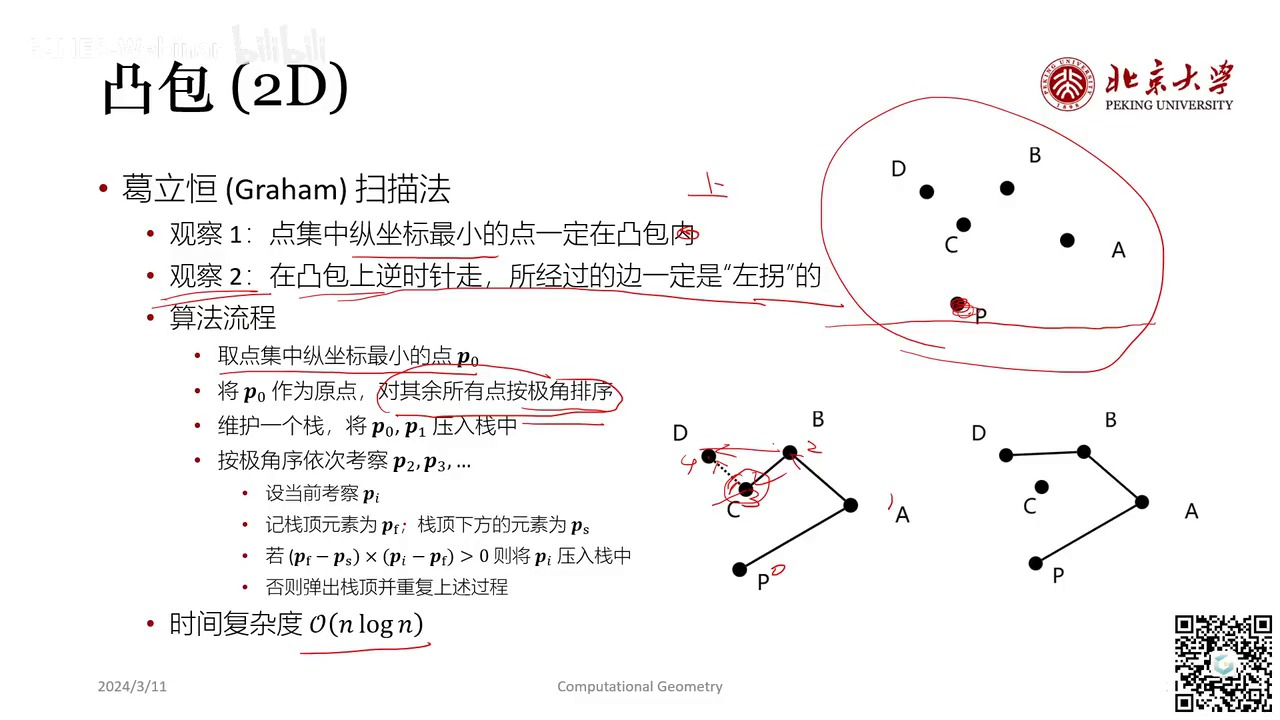
\includegraphics[width=0.92\textwidth]{figures/fig_18_graham.jpg}
\caption{葛立恒扫描法：手写演示从 $P$ 出发按极角考察 $A,B,C,D$，非左拐时弹栈\vtag}
\end{figure}
\srcnote{01:03:15--01:03:30}
\end{minipage}


\subsection{三维凸包：增量法}

三维凸包可用增量法构造。给定前 $n-1$ 个点的凸包，考察新点的加入：若新点在凸包内（用前面的点与凸多面体判断），凸包不变；若新点不在凸包内，就以新点为光源向凸包发射光线，被照亮的面与未被照亮的面之间形成明暗分界线。删除被照亮的面，再连接光源与分界线上的边，形成新的凸包。

每加入一个点都要检查它与每个面的关系，因此时间复杂度为 $O(n^2)$。多点共面时，可以对输入点做随机扰动。三维凸包的其它算法有：

\begin{itemize}
\item \textbf{暴力法}：枚举 $\binom n3$ 个三角形，若其余所有点都在某个三角形的同一侧，它就在凸包上。
\item \textbf{快速凸包}（quick hull）：增量法的变种，每次选择离当前凸包最远的点加入。实现并不容易，但许多开源计算几何库都已提供，三角剖分也一样，可以直接调用。
\end{itemize}

\noindent\begin{minipage}{\textwidth}
\begin{figure}[H]
\centering
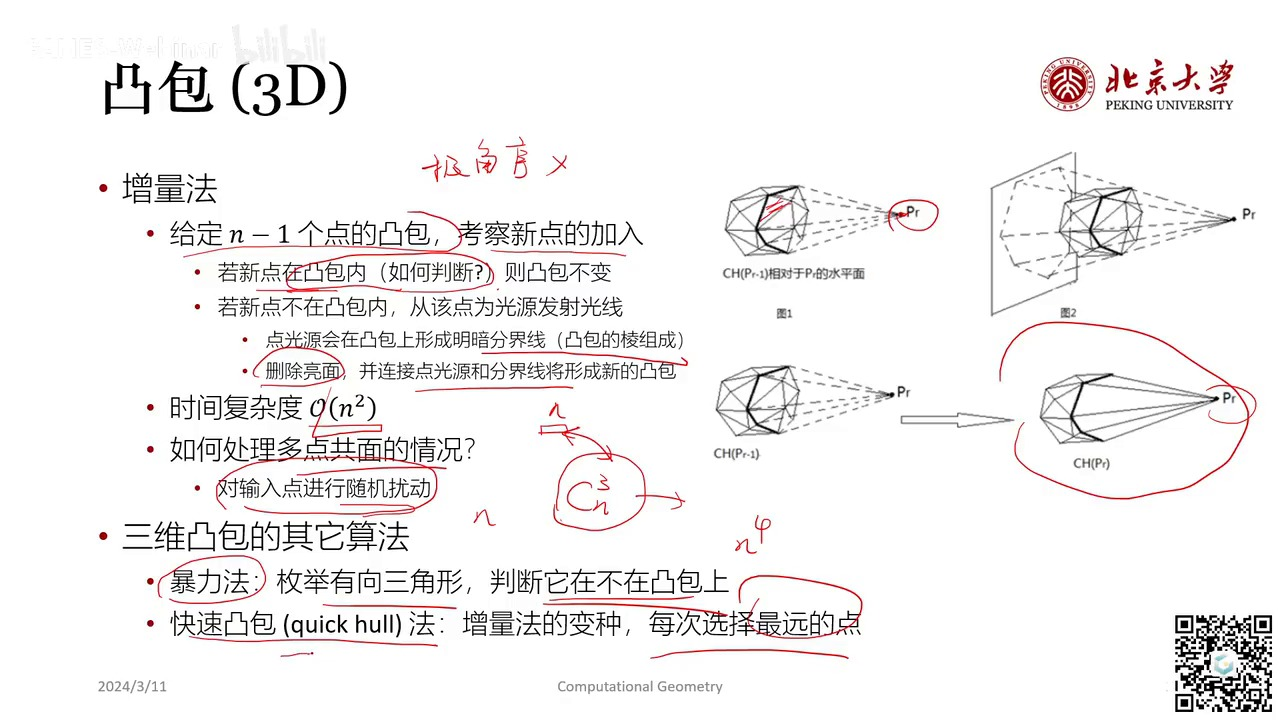
\includegraphics[width=0.92\textwidth]{figures/fig_19_hull3d.jpg}
\caption{三维凸包增量法：新点作为光源，删除被照亮的面并连接明暗分界线\vtag}
\end{figure}
\srcnote{01:07:00--01:07:15}
\end{minipage}


\section{平面最近点对与最小圆覆盖}

\subsection{分治求平面最近点对}

求平面点集中距离最近的两点，暴力法需要 $O(n^2)$。分治算法将点集 $S$ 沿中线划分为两个子集 $S_1,S_2$，此时最近点对只有三种可能：在 $S_1$ 内、在 $S_2$ 内，或横跨 $S_1$ 和 $S_2$。前两种递归求解。对于第三种，设 $S_1$、$S_2$ 的最近点对距离分别为 $h_1,h_2$，只需考虑到中线的距离小于
\[
h=\min(h_1,h_2)
\]
的点，它们构成带状集合 $B$。在 $B$ 内按 $y$ 坐标排序扫描，每个点只需与 $y$ 方向距离小于 $h$ 的少数几个点比较。

\noindent\begin{minipage}{\textwidth}
\begin{figure}[H]
\centering
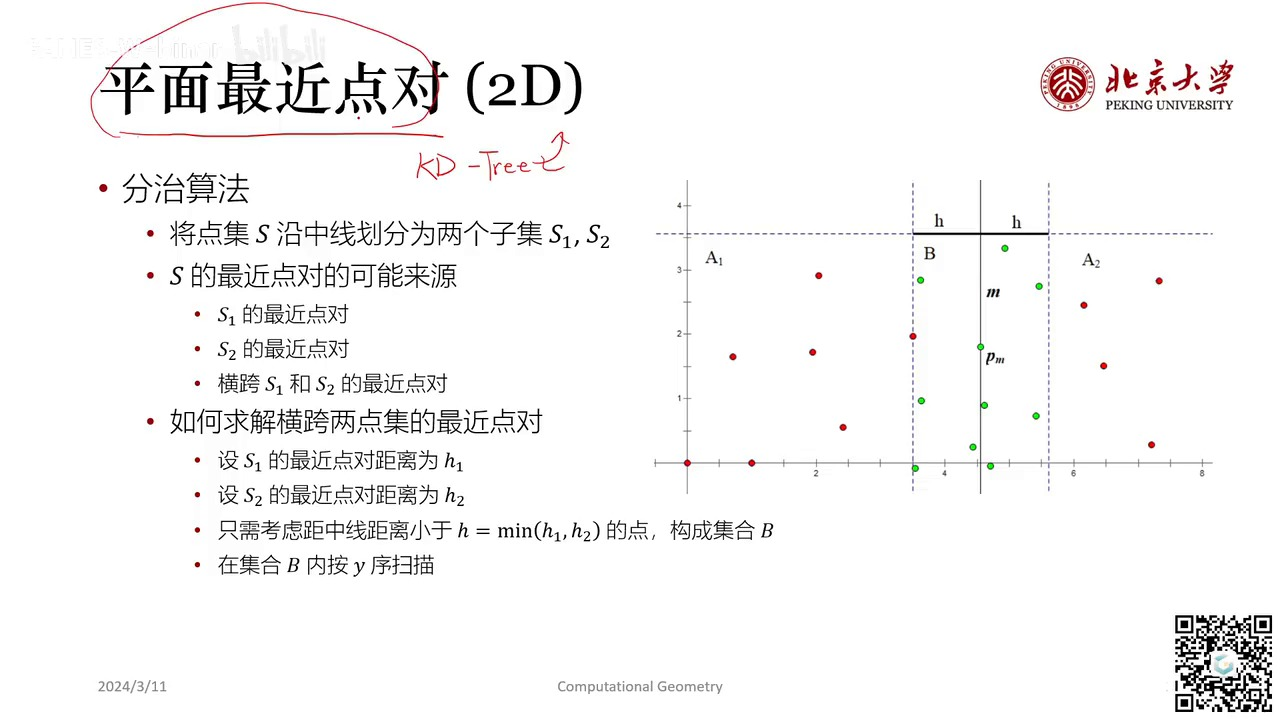
\includegraphics[width=0.92\textwidth]{figures/fig_20_closest_pair.jpg}
\caption{平面最近点对的分治算法：沿中线划分，只在宽为 $2h$ 的带状区域内跨界比较\vtag}
\end{figure}
\srcnote{01:07:45--01:08:00}
\end{minipage}


\subsection{最小圆覆盖的性质}

如果说包围盒对应的是凸包，那么“包围球”（二维中是圆）对应的就是最小圆覆盖：包围给定点集的\emph{唯一}最小的圆。它有几条性质：凸包一定在最小覆盖圆内；最小覆盖圆只有三种情况，即
\begin{itemize}
\item 圆心在某一点处，半径为零（点集只有一个点）；
\item 圆心在两点的中点，直径为两点间的距离；
\item 圆心为三点的外心，半径为外接圆半径。
\end{itemize}

最小圆覆盖还有增量构造的性质，与凸包类似：给定前 $n-1$ 个点的最小覆盖圆，第 $n$ 个点要么在圆内，此时圆不变；要么在圆外，此时新的最小覆盖圆\emph{必须经过该点}，因为没有比它更靠外的点了。

\noindent\begin{minipage}{\textwidth}
\begin{figure}[H]
\centering
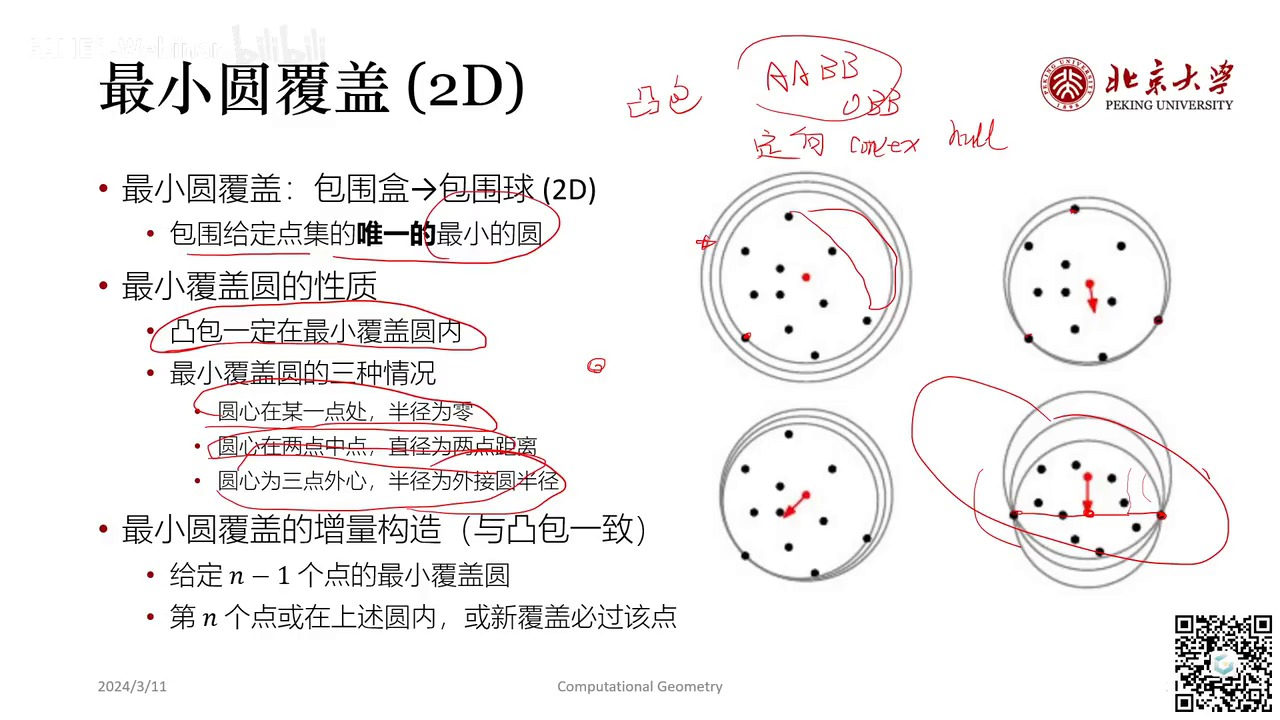
\includegraphics[width=0.92\textwidth]{figures/fig_21_min_circle_cases.jpg}
\caption{最小覆盖圆的三种情况与增量构造\vtag}
\end{figure}
\srcnote{01:10:30--01:10:45}
\end{minipage}


\subsection{随机增量法}

利用上面的性质，可以写出三层循环的随机增量算法（先把点随机打乱）：

\begin{enumerate}
\item $\odot_{\text{ans}}=\mathrm{Circle}(\mathbf p_1)$。
\item For $i=2\to n$：若 $\mathbf p_i\in\odot_{\text{ans}}$，直接进入下一次循环；否则令 $\odot_{\text{ans}}=\mathrm{Circle}(\mathbf p_i)$，并且：
  \begin{enumerate}
  \item For $j=1\to i-1$：若 $\mathbf p_j\in\odot_{\text{ans}}$，进入下一次循环；否则令 $\odot_{\text{ans}}=\mathrm{Circle}(\mathbf p_i,\mathbf p_j)$，并且：
    \begin{enumerate}
    \item For $k=1\to j-1$：若 $\mathbf p_k\in\odot_{\text{ans}}$，进入下一次循环；否则 $\odot_{\text{ans}}=\mathrm{Circle}(\mathbf p_i,\mathbf p_j,\mathbf p_k)$。
    \end{enumerate}
  \end{enumerate}
\end{enumerate}

第二层循环得到的圆一定过 $\mathbf p_i$，第三层得到的圆一定同时过 $\mathbf p_i$ 和 $\mathbf p_j$；三个点就能直接确定外接圆。

\noindent\begin{minipage}{\textwidth}
\begin{figure}[H]
\centering
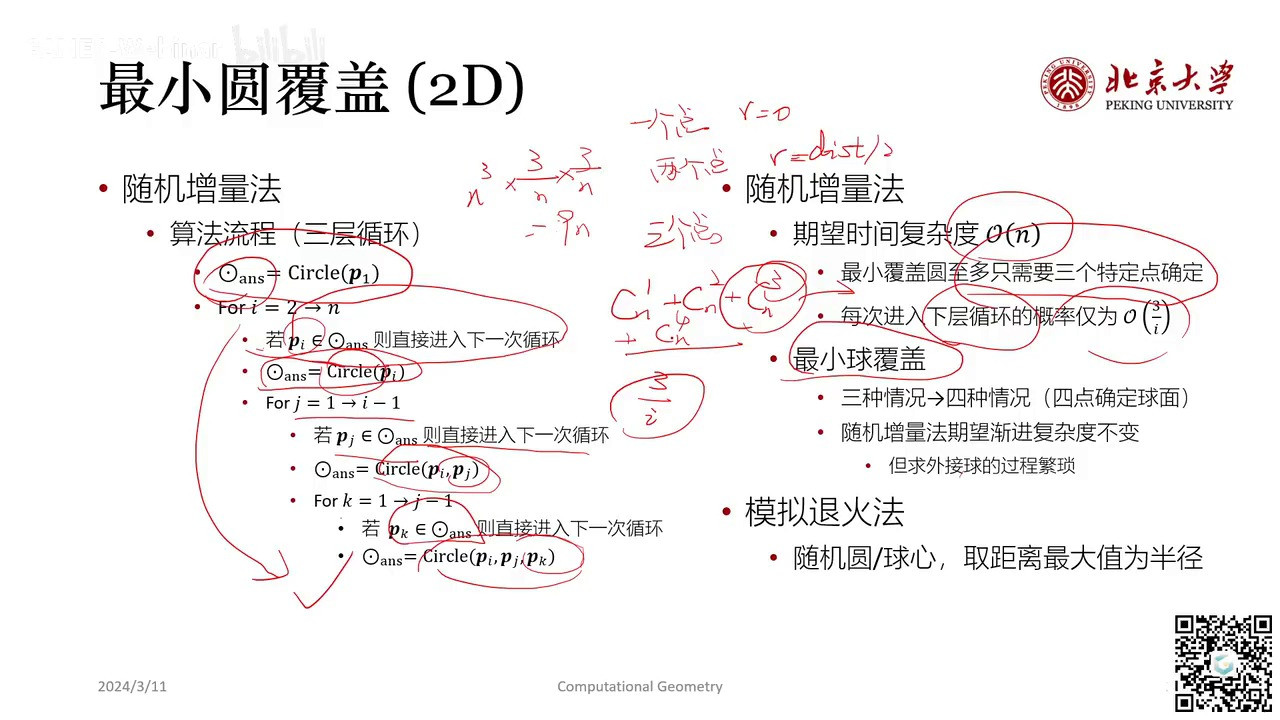
\includegraphics[width=0.92\textwidth]{figures/fig_22_min_circle_algo.jpg}
\caption{随机增量法的三层循环，以及讲者手写的期望复杂度推导\vtag}
\end{figure}
\srcnote{01:15:30--01:15:45}
\end{minipage}


三层循环看起来是 $O(n^3)$，为什么期望复杂度是线性的？若暴力枚举，需要检查 $\binom n1+\binom n2+\binom n3$ 个候选圆。随机增量法的关键在于：最小覆盖圆至多只由三个特定点确定。在前 $i$ 个点中，第 $i$ 个点恰好是这三个点之一的概率至多为 $3/i$，所以进入下一层循环的概率只有
\[
P(\text{进入下一层})\le\frac{3}{i}=O\!\left(\frac{3}{i}\right).
\]
第三层每次花 $O(j)$，进入概率 $3/j$，期望 $O(1)$；第二层每次期望 $O(i)$，进入概率 $3/i$，期望 $O(1)$。讲者在手写板上把这个推导写成 $n\cdot\frac3n\cdot\frac3n\cdot n^2$ 量级的乘积，最终得到的总代价是 $9n$ 量级，所以期望时间复杂度为 $O(n)$。

\begin{practicebox}{推广与替代}
\begin{itemize}
\item \textbf{最小球覆盖}：三种情况变为四种，第四种是由四个点确定的球面。进入下一层的概率仍是同一量级，所以随机增量法的期望复杂度不变，只是求外接球的过程繁琐一些。
\item \textbf{模拟退火}：随机选取圆心（球心），以到各点距离的最大值为半径，逐步向半径更小的方向移动。它是近似方法，但实现简单。
\item \textbf{动手验证}：把三层循环实现出来，统计第三层循环的实际执行次数，看它随 $n$ 增长是否接近线性。
\end{itemize}
\end{practicebox}

\noindent\begin{minipage}{\textwidth}
\begin{figure}[H]
\centering
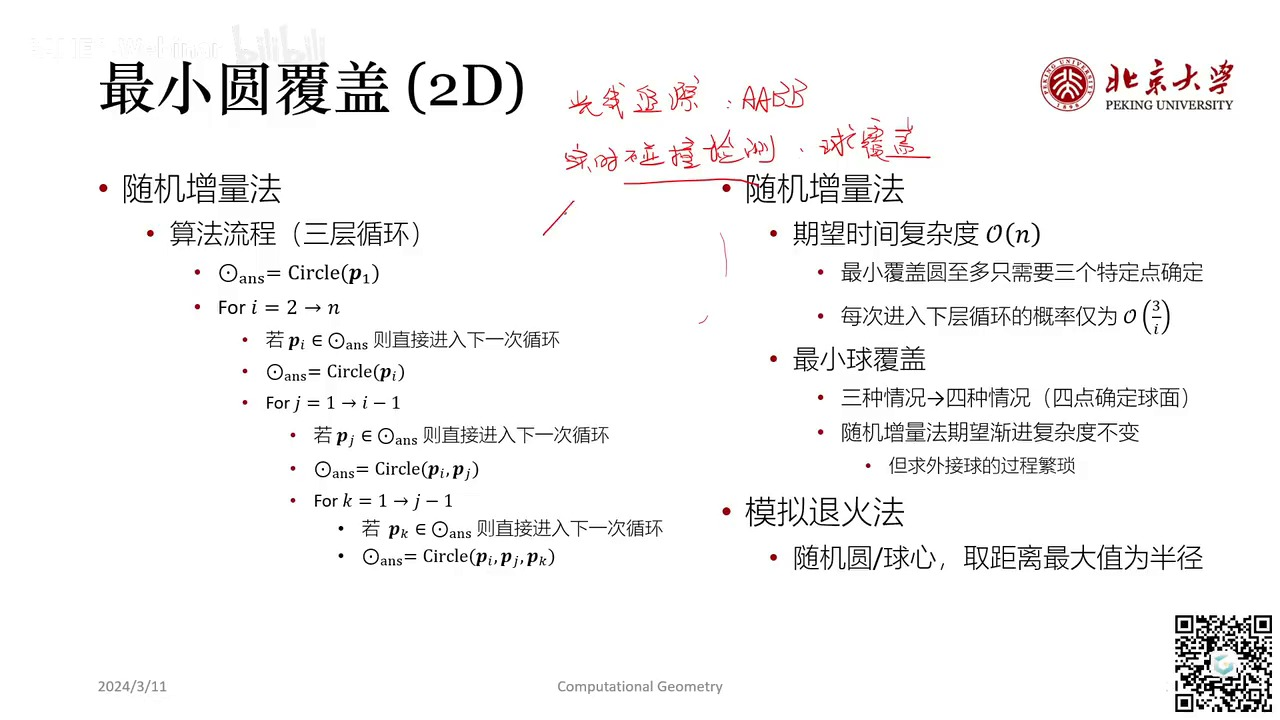
\includegraphics[width=0.92\textwidth]{figures/fig_23_min_circle_complexity.jpg}
\caption{最小圆覆盖的期望复杂度与最小球覆盖、模拟退火\vtag}
\end{figure}
\srcnote{01:19:15--01:19:30}
\end{minipage}


\begin{importantbox}{包围体在碰撞检测中的作用}
最小球覆盖与前面的三角形距离直接相关。要判断两大片三角形网格是否碰撞，最精确的办法是求它们的凸包，粗一些的是 AABB 或 OBB，最常用的是包围球。对两个球做碰撞检测最容易：比较球心距离与半径之和即可。图形学中常把一簇三角形先用球包起来，球不相交，里面的三角形就不必再逐对检查。
\end{importantbox}

\section{反演变换}

\subsection{点的反演与圆的反演}

最后一个主题是反演（inversion）。给定反演中心 $\mathbf o$ 和反演半径 $r$，若 $\mathbf o,\mathbf p,\mathbf p'$ 三点共线（$\mathbf p'$ 在射线 $\mathbf o\mathbf p$ 上），且
\[
\|\mathbf p-\mathbf o\|\,\|\mathbf p'-\mathbf o\|=r^2,
\]
则称 $\mathbf p$ 与 $\mathbf p'$ 互为反演点。由此立即得到：圆 $\mathbf o$ 外的点，其反演点在圆内；圆内的点，其反演点在圆外。

过反演中心的圆反演后变成直线。以 $\mathbf o$ 为原点，设圆的方程为
\[
(x-x_0)^2+(y-y_0)^2=a^2,\qquad x_0^2+y_0^2=a^2,
\]
其中第二个式子表示圆过原点。课件给出的反演关系写成
\[
(x,y)\to(x',y')=\left(\frac{r^2}{x},\frac{r^2}{y}\right),
\]
把它代入圆的方程联立，就得到反演后的直线方程；反过来，不过反演中心的直线反演后是过反演中心的圆。

\noindent\begin{minipage}{\textwidth}
\begin{figure}[H]
\centering
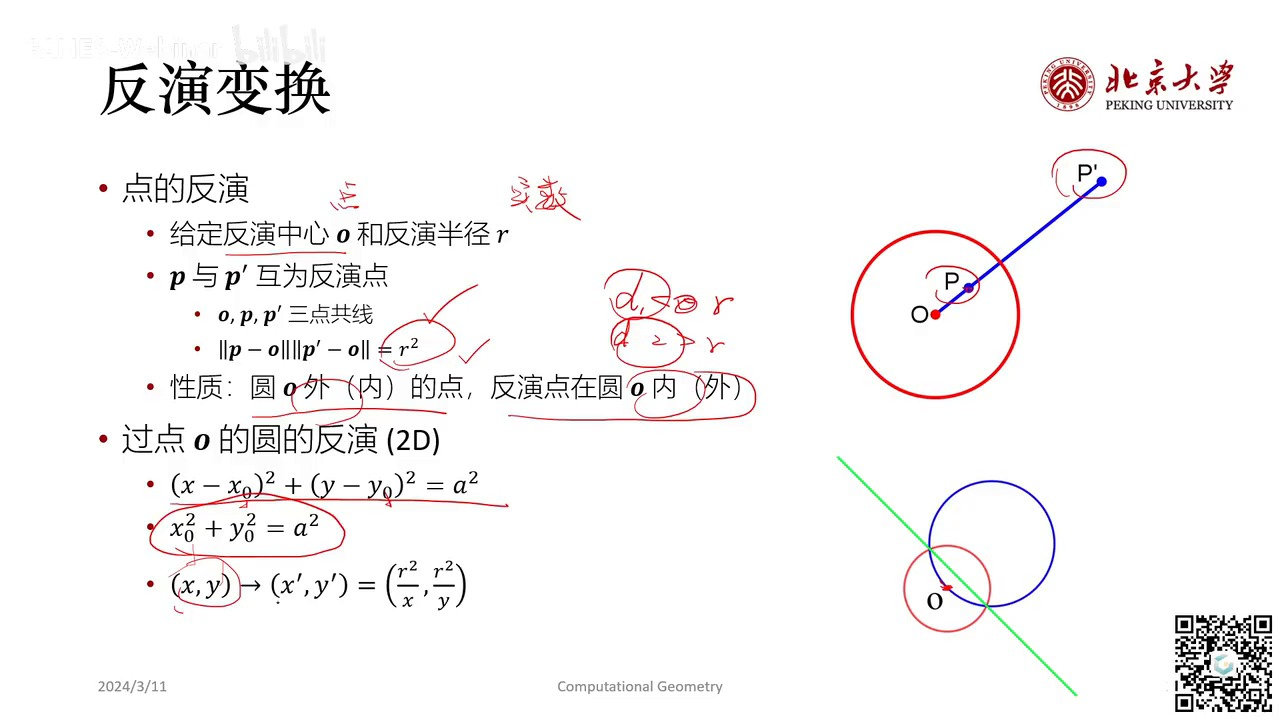
\includegraphics[width=0.92\textwidth]{figures/fig_24_inversion.jpg}
\caption{点的反演与过反演中心的圆的反演：红色反演圆，蓝色圆反演为绿色直线\vtag}
\end{figure}
\srcnote{01:22:00--01:22:15}
\end{minipage}


\begin{warningbox}{坐标反演公式的写法}
讲义作者提醒：按定义 $\|\mathbf p\|\,\|\mathbf p'\|=r^2$ 且 $\mathbf p'$ 与 $\mathbf p$ 同向，正确的坐标公式是
\[
(x',y')=\frac{r^2}{x^2+y^2}\,(x,y),
\]
而不是逐分量取倒数。课件中的 $(r^2/x,\ r^2/y)$ 只能看作简写，实际推导时应使用上式。用它代入 $x^2+y^2=2x_0x+2y_0y$，可得直线 $2x_0x'+2y_0y'=r^2$。
\end{warningbox}

\subsection{反演的应用与意义}

不过反演中心的圆，反演后仍是不过反演中心的圆。这一性质的典型应用是：求过两圆外一点、并与两圆都相切的所有圆。直接求解要联立复杂的相切条件；以该点为反演中心做反演后，所求的圆变成直线，两个已知圆仍是圆，问题就变成求两圆的公切线，再反演回去即可。

反演可以推广到三维，圆对应球，直线对应平面。它的意义在于：反演是几何图形关于球的“镜像”。普通镜像中间是一个平面，左边一点经过镜面得到右边的对称点；反演则以球面为镜子，球内一点映到球外。在微分方程求解中，静电学里的“电像法”就是利用这种镜像：用球外的一个虚拟电荷代替导体球对电场的影响。

\noindent\begin{minipage}{\textwidth}
\begin{figure}[H]
\centering
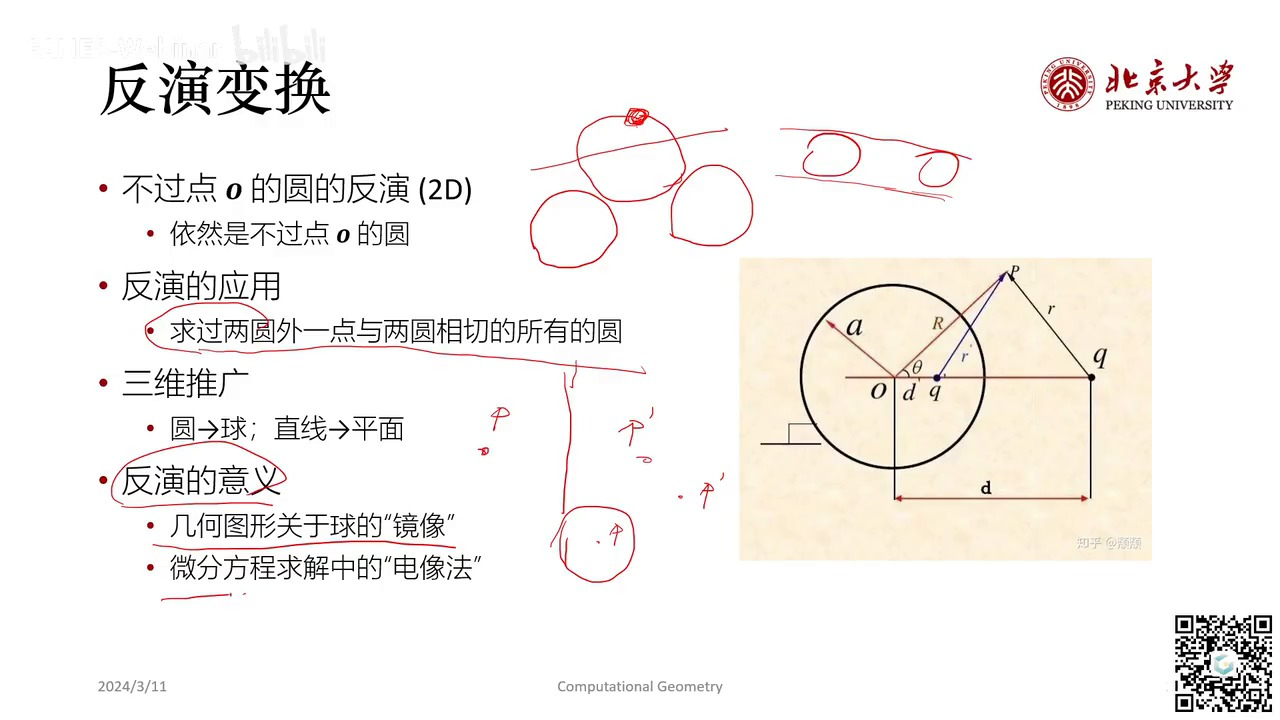
\includegraphics[width=0.92\textwidth]{figures/fig_25_inversion_apps.jpg}
\caption{反演的应用：求过一点并与两圆相切的圆；三维推广与“镜像”意义\vtag}
\end{figure}
\srcnote{01:24:30--01:24:45}
\end{minipage}


\section{总结与课后练习}

讲者推荐了三份参考资料：Mark de Berg 等著、邓俊辉译的《计算几何：算法与应用》（第 3 版，清华大学出版社，2009）；周培德的《计算几何：算法设计与分析》（清华大学出版社，2005）；以及王华民老师 GAMES103 的第 9 讲，后者讲的碰撞检测与本讲的三角形距离密切相关。

课后练习选自北京大学在线评测系统 POJ，在任何搜索引擎上搜 POJ 都能找到。这些都是讲者以前刷过的题，有易有难。课程不会考核这部分内容，因为计算几何本身已经是图形学的一部分，不算特别“数学”的内容。

\begin{itemize}
\item 点、线、面：2318, 2398, 3304, 1269, 2653, 1066, 1410, 1696, 3449, 1584, 2074；
\item 凸包：1113, 2007, 1228, 3348；
\item 圆、球：1375, 1329, 2354, 1106, 1673。
\end{itemize}

\noindent\begin{minipage}{\textwidth}
\begin{figure}[H]
\centering
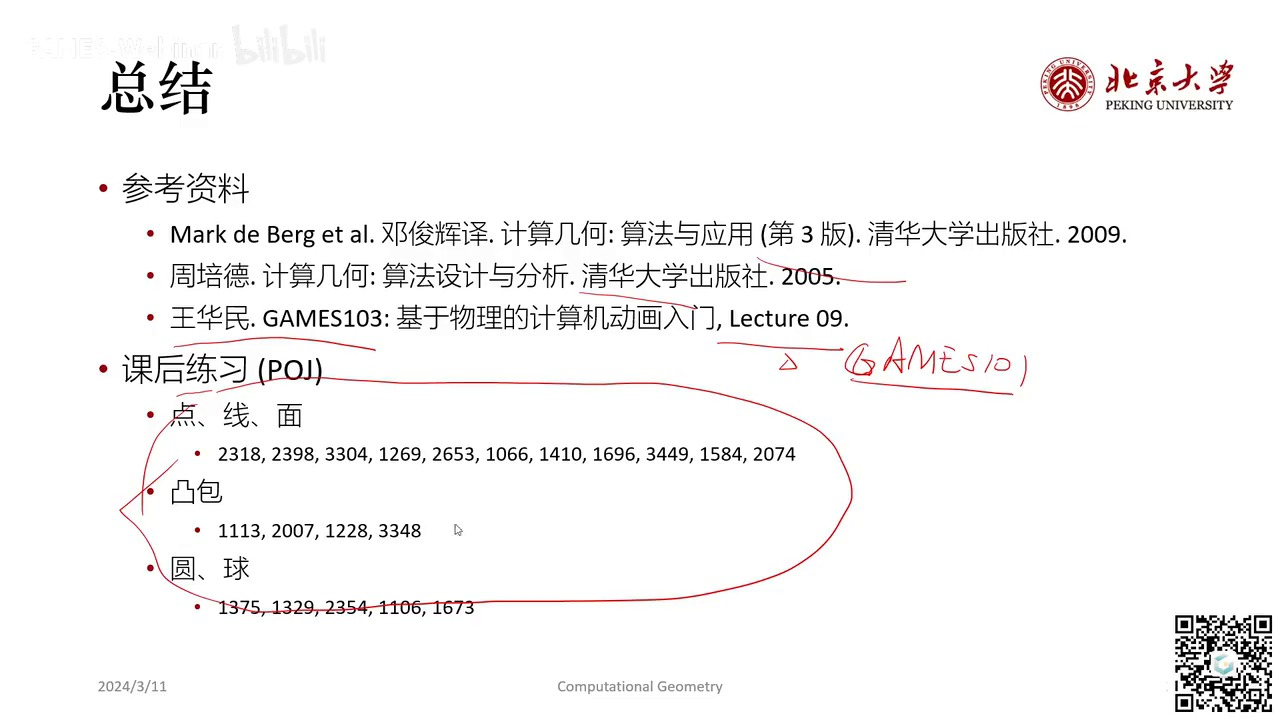
\includegraphics[width=0.92\textwidth]{figures/fig_26_summary.jpg}
\caption{总结页：参考资料与 POJ 课后练习题号\vtag}
\end{figure}
\srcnote{01:29:15--01:29:30}
\end{minipage}


\begin{practicebox}{自测清单}
\begin{itemize}
\item 用叉乘写出点到直线的距离，并说明为什么点到射线需要分 $t\ge0$ 与 $t<0$ 两种情况。
\item 写出线段跨立测试的 $s_1,s_2$，说明取等号对应什么情况，以及它为什么不需要除法。
\item 用有向面积求任意多边形的面积，并解释参考点取在多边形外时为什么结果仍然正确。
\item 光线投射法遇到射线经过顶点时如何处理？
\item 为什么三维三角形之间的距离要比较 6 组点—面和 9 组边—边，而二维只需 6 组点—面？
\item 写出葛立恒扫描法的“左拐”判据，并说明 $O(n\log n)$ 的瓶颈在哪里。
\item 解释最小圆覆盖随机增量法为什么期望是线性时间。
\end{itemize}
\end{practicebox}

下一讲开始，课程内容会与图形学结合得更紧密。

\end{document}
